\newcommand{\docklasse}{article}			% vælg report eller article
\newcommand{\AbstractVisible}{false}		% Resumé på forside
\newcommand{\HandindateVisible}{false}		% Afleveringsdato på forside
\newcommand{\GroupVisible}{false}			% Gruppenummer på forside
\newcommand{\NamesVisible}{true}			% Navne og mails på forside
\newcommand{\danish}{false}					% true=dansk rapport, false=engelsk rapport

\documentclass[11pt,a4paper]{\docklasse}	% Vælg article eller report
\NeedsTeXFormat{LaTeX2e}[1994/12/01]		% Angiver hvilken LaTeX distribution, der er minimum
\usepackage[utf8]{inputenc}					% Giver adgang til specialtegn som æ, ø og å
\usepackage[T1]{fontenc}					% Giver outputformateringen af skriften
\RequirePackage{ifthen}
\newcommand{\hvisdansk}[2]{\ifthenelse{\equal{\danish}{true}}{#1}{#2}}
\def\ifdanish{\equal{\danish}{true}}
\hvisdansk%
{\usepackage[english,danish]{babel}}%		% Dansk sprogformatering som 1. prioritet, dernæst engelsk
{\usepackage[danish,main=UKenglish]{babel}}				% Afsnitsbetegnelse, datoformatering  osv.
											% english bruges til bl.a. \mathbb{}
% Under Options>Configure Texmaker>Commands skal "Makeindex" feltet ændres til "makeindex %.nlo -s nomencl.ist -o %.nls -t %.nlg" (Dette for at kunne bruge nomenclature)
% For renere/mere overskuelige filmapper skal der sættes flueben i "Use "build" subdirectory for output files
% Når dette flueben er sat skal man også ændre skrives "build\" foran alle %-tegnene under "Bib(la)tex" og "Makeindex"


% ==================================================================
% ============== Generelt ==========================================
% ==================================================================

\usepackage{forloop}		% Giver mulighed for at lave forløkker

\usepackage{totcount}		% Giver mulighed for at referere til counterens sidste værdi
\newtotcounter{BilagSider}	% Bruges til informationssiden
\usepackage[inline]{enumitem} % inline enum list

% Farver
\usepackage{color}

% Manuel fastsættelse af floatnummereringens dybde
%\numberwithin{figure}{chapter}
%\numberwithin{equation}{section}
%\numberwithin{table}{chapter}

% Opsætning af linjeafstand
%\usepackage{setspace}		% Derefter kan der løbende kaldes \singlespacing, \onehalfspacing eller \doublespacing
							% Disse kan også kaldes i miljøer, f.eks. \begin{onehalfspace}, \begin{spacing}{2.5}

% For mere kontrol kan linjeafstand og andre afstande opsættes manuelt
% Det er muligt at definere afstandende med plus og/eller minus margin <længde> plus <ekstra længde> minus <mindre længde>
%\setlength{\baselineskip}{<længde>}	% Linjeafstand
%\setlength{\parskip}{<længde>}			% Afsnitsafstand
%\setlength{\parindent}{<længde>}		% Indrykning af første linje

% (Obs. den aktuelle afstand kan printes ved at skrive \the\<afstandsparameter>

% Nummerering af subsubsection
\setcounter{secnumdepth}{3}
\renewcommand{\thesubsubsection}{\thesubsection .\arabic{subsubsection}}
%\setcounter{tocdepth}{3}		% Denne kan indkommenteres, hvis subsubsections ønskes i indholdsfortegnelsen

%\usepackage[all]{nowidow}		% Kan fjerne horeunger, hvis de er et problem

% ==================================================================
% ============== Referencer og links ===============================
% ==================================================================
% Hyperref laver referencer om til linkede referencer og hyperlink samt laver bogmærker
% Brug \href{<url>}{<Tekst der printes>} til at lave hyperlinks
% Der kan refereres til et tilfældigt stykke tekst vha. \hypertarget{<label>}{<target caption>} og \hyperlink{<label>}{<link caption>}

\PassOptionsToPackage{hyphens}{url}\usepackage[	% \PassOptionsToPackage{hyphens}{url} tillader line-breaking af lange url'er
			bookmarks=true			% Viser bookmarks når pdf'en åbnes
			,colorlinks=true		% true=farvede links, false(default)=farvede rammer
			,linkcolor=red
			,citecolor=green
			,filecolor=magenta
			,urlcolor=blue
			,hidelinks				% Fjerner rammer og farve (udkommenteres for at aktivere farvede links)
			,bookmarksnumbered
			,breaklinks=true
			]{hyperref}
\usepackage{bookmark}
			

%\newcommand{\tref}[2]				% \tref{Test}{eq:lign} vil give outputtet Test 2 (hvis eq:lign refererer til ligning 2), hvor både "Test" og "2" er links.
%		{\hyperref[#2]{#1~\ref*{#2}}}
	

%\usepackage{cleveref}				% Alternativ referencepakke. Kan bl.a. bruges til \crefrange{<1. label>}{<2. label>}, men den kræver opsætning.



% ==================================================================
% ============== Marginer og headings ==============================
% ==================================================================
% Marginer og sidehoved- / -fodstørrelse
\usepackage	[a4paper,
			includeheadfoot,
			head=1.8cm,
			foot=.5cm,
			headsep=.5cm,
			footskip=1cm,
			bindingoffset=0cm,
			top=.7cm,
			bottom=2cm,
			inner=2.5cm,
			outer=2.5cm,
			marginparsep=0.5cm,
			marginparwidth=2.4cm,
			twoside
			]{geometry}	

\savegeometry{A4ligemargen}		% Gemmer indstillinger til forside

\geometry{inner=2.5cm,
		  outer=3.5cm}
\savegeometry{A4uligemargen}	% Gemmerindstillinger for uens margen

\geometry{paperwidth=420mm}
\savegeometry{A3}				% Gemmerindstillinger for bredere side
\geometry{paperwidth=590mm}
\savegeometry{A4x3}				% Gemmerindstillinger for endnu bredere side

\loadgeometry{A4uligemargen}	% Lige-/uligemargen samt A3/A4x3 kan hentes med \loadgeometry{<>}
								% OBS. kaldes A3 eller A4x3 skal der først kaldes
								% \eject \pdfpagewidth=<420 eller 590>mm \pdfpageheight=297mm
								% \titlespacing*{\chapter}{1cm}{0cm}{1cm}[<22 eller 39>cm]
								% Når man derefter skifter tilbage skal der nulstilles til
								% \eject \pdfpagewidth=210mm \pdfpageheight=297mm
								% \titlespacing*{\chapter}{1cm}{0cm}{1cm}[1cm]

%\usepackage{marginnote}		% Bruges hvis marginnoter skal placeres i en bestemt højde eller i et float-miljø.
								% Syntaks: \marginnote{<Tekst m.m.>}[<lodret offset>]

\newcommand{\blankside}[1][]{%	% Kodeblok til at lave en blank bagside på 2-sidet format
			\thispagestyle{empty}
			\ 
			\vspace{9cm}
			\begin{center}
			#1
			\end{center}
			\clearpage
			\thispagestyle{fancy}}

% Indhold i sidehoved / -fod
\usepackage{lastpage}			% Bruges til at referere til sidste sidenummer
\usepackage{fancyhdr}
	\pagestyle{fancy}
% Sidehoved
	\fancyhead[LO,RE]{}			% Indvendig
	\fancyhead[CO,CE]{}			% Midt
	\fancyhead[RO,LE]{}			% Udvendig		
% Sidefod
	% Indvendig% \leftmark kan ændres til \rightmark, hvis der ønskes sectionnavne
\newcommand{\StandardFooter}{
	\fancyhead[LO]{\parbox[t][0mm][t]{11cm}{\raggedright\leftmark}}
	\fancyhead[RE]{\parbox[t][0mm][t]{11cm}{\raggedleft\leftmark}}
	\fancyfoot[CO,CE]{}								% Midt
	\fancyfoot[RO,LE]{\ifthenelse{\ifdanish}{Side \thepage\ af \pageref{LastPage}}{Page \thepage\ of \pageref{LastPage}}}	% Udvendig
}
\StandardFooter
% Hvis der vælges 1-sidet format, kan sidehovedet/-fod kaldes med \chead{}, \rhead{}, \lhead{}, \cfoot{}, \rfoot{}, \lfoot{}	

% Streger
	\renewcommand{\headrulewidth}{0.5pt}	% Tykkelse af topstreg
	\renewcommand{\footrulewidth}{0.5pt}	% Tykkelse af bundstreg

	\fancypagestyle{plain}		% Lav fancyheader på sider med chapter
	
% Dermed kan billeder indsættes (umiddelbart efter section-/chaptertitlen) vha. f.eks.
% \chead{\includegraphics[height=1.7cm]{<filnavn>}
% OBS! Med disse opsætninger må figurhøjden ikke overstige 1.7cm.


% ==================================================================
% ============== Chapterformatering ================================
% ==================================================================	
\usepackage{titlesec}			%Muliggør formatering af chaptertitler, sectionstitler osv.

\titleformat{\chapter}
			[frame]	% Kapitel type
			{\normalfont}				% Generel formatering
			{\filright					% Venstrejusteret
				\footnotesize			% Tekststørrelse af kapitellabel
				\enspace				% Afstand før kapitellabel
				\chaptername~\thechapter		% Kapitellabel
				\enspace}				% Afstand efter kapitellabel
			{8pt}						% Afstand mellem ramme og titel
			{\Large\bfseries\filcenter}	% Titelformatering

\titlespacing*{\chapter}		% Afstand omkring chaptertitler (* fjerne indrykning på første linje)
  {1cm}{0cm}{1cm}[1cm]			% {venste}{før}{efter}[højre}
  
  
% ==================================================================
% ============== Bilag =============================================
% ==================================================================
\newcommand{\startbilag}{		% Kommandoen kaldes i main og opsætter formateringen af bilag
	\clearpage
	\appendix
	\ifthenelse{\equal{\docklasse}{report}}
		{\hvisdansk%
			{\renewcommand{\chaptername}{Bilag}}%
			{\renewcommand{\chaptername}{Appendix}}%
		}%
		{}
	\clearpage
	\ifthenelse{\equal{\docklasse}{report}}%
		{\hvisdansk%
			{\addcontentsline{toc}{chapter}{Bilag}}%
			{\addcontentsline{toc}{chapter}{Appendices}}}%
		{\phantomsection\hvisdansk%
			{\addcontentsline{toc}{section}{Bilag}}%
			{\addcontentsline{toc}{section}{Appendices}}}%
	\chead{}
	\hvisdansk{	
	\fancyhead[RO]{\raggedleft BILAG}\fancyhead[LE]{\raggedright BILAG}}{
	\fancyhead[RO]{\raggedleft APPENDIX}\fancyhead[LE]{\raggedright APPENDIX}}
	}
%
% ==================================================================
% ============== Ord- og symbolliste ===============================
% ==================================================================
% For at anvende disse skal man først compile (F6) dernæst MakeIndex (F12) og så compile igen
% Syntaks: \nm[<gruppe>]{<Ord/Symbol>}{<Forklaring\nomunit[<værdi>]{<enhed>}>}
%	gruppe: O for ord, K for konstant, V for variabel
%	Ord/Symbol: Ord/Symbol der skal i listen
%	Forklaring: Kort forklaring af ordet/symbolet evt. med enheder
%	\nomunit kan kaldes hvis der skal enhed på konstanter og variable. <værdi> er konstanters værdi og er optional

% Brug \printnomenclature til at oprette symbollisten 
\hvisdansk%
		{\usepackage[danish,							% Dansk syntakt
%					intoc,								% I indholdsfortegnelse (Ønskes der nummereret kapitel indsættes i stedet nedenstående kodeblok i dokumentet)
					refpage								% Tilføjer sidereferencer
					]{nomencl}}%
		{\usepackage[english,							% Engelsk syntakt
%					intoc,								% I indholdsfortegnelse (Ønskes der nummereret kapitel indsættes i stedet nedenstående kodeblok i dokumentet)
					refpage								% Tilføjer sidereferencer
					]{nomencl}}			
							
			
% OBS!!! For at bruge denne skal MakeIndex-feltet under Commands i Configure Texmaker ændres til
% makeindex %.nlo -s nomencl.ist -o %.nls -t %.nlg

% Kodeblok til nummereret kapitel (Indsættes i stedet for \printnomenclature)
%\let\stdchapter\chapter
%\def\chapter*#1{\stdchapter{#1}}
%\printnomenclature
%\let\chapter\stdchapter

% Aktiver ordliste
\makenomenclature

% Listens navn	
\hvisdansk{\renewcommand{\nomname}{Symbolliste og ordforklaring}}{\renewcommand{\nomname}{Symbols and Nomenclature}}

% Linjeafstand
\setlength{\nomitemsep}{-1pt}

% Der oprettes en ny og kortere kommando \nm der også tjekker om der er tale om et ord
\RequirePackage{scrextend}
\newcommand{\nm}[3][]{
	\ifthenelse{\equal{#1}{O}}
		{\marginpar{\ifthispageodd{}{\flushright}\vspace{-.5\baselineskip}\textbf{\footnotesize #2}}\hspace{-.35em}\nomenclature[C]{#2:}{#3}}%		% Hvis det er et ord, skrives ordet også i marginen
	{\ifthenelse{\equal{#1}{V}}{\nomenclature[A]{#2}{#3}}
	{\ifthenelse{\equal{#1}{S}}{\nomenclature[B]{#2}{#3}}
	{\nomenclature[#1]{#2}{#3}}}}}											% Ønskes dette ikke, kan det erstattes med \newcommand{\nm}[3][*]{\nomenclature[#1]{#2}{#3}}

% Gruppering
	\RequirePackage{ifthen}
	\renewcommand{\nomgroup}[1]{
		\item[]\hspace*{-\leftmargin}							% Fjerner indrykning
		\rule[2pt]{0.43\linewidth}{1pt}\hfill					% Streg før
		 	\ifthenelse{\equal{#1}{A}}{\parbox[c][10mm][c]{0.2\linewidth}{\centering\textbf{\hvisdansk{Konstanter og variabler}{Constants \& Variables}}}}{	% 1. gruppes overskrift
 		 	\ifthenelse{\equal{#1}{B}}{\textbf{\hvisdansk{Andre symboler}{Other Symbols}}}{% 3. gruppes overskrift
 		 	\ifthenelse{\equal{#1}{C}}{\textbf{\hvisdansk{Ordforklaring}{Nomenclature}}}{			% 4. gruppes overskrift
 			\textbf{Fejl index}}}}								% Default gruppes overskrift
		\hfill\rule[2pt]{0.43\linewidth}{1pt}}					% Streg efter

% Enheder. Indsættes til sidst i symboldefinitionen
% Syntaks: \nomunit[<værdi af konstant>]{<enheder>}
% Skal ikke skrives i mathmode
	\newcommand{\nomunit}[2][]{%
		\renewcommand{\nomentryend}{\hspace*{\fill} \footnotesize \ensuremath{\textstyle #1\,\mathrm{\left[#2\right]}}}}


% ==================================================================
% ============== Kildekode =========================================
% ==================================================================
% Denne pakke bruges til at opsætte og genkende kildekode.
% Pakken genkender selv kommentarer og kommandoer, og giver det særlig formatering.
% Manglende kommandoer kan tilføjes og ligeledes kan forkerte kommandoer fjernes
% Koden kan indsættes manuelt i et lstlisting miljø, som inline kode vha. \lstline!<kode>! eller hentes ind fra en fil vha.
% \lstinputlisting[language=Python, firstline=37, lastline=45]{source_filename.py}

% Der defineres tre farve, der bruges til formatering af koden.
\definecolor{mygreen}{RGB}{0,110,0}
\definecolor{mygray}{RGB}{100,100,100}
\definecolor{myorange}{RGB}{205,130,18}
\definecolor{mymauve}{RGB}{148,0,209}
\usepackage{listings}
\lstset{ %				% Opsætning af kodeformateringen. De første options er de vigtige.
	language = [visual]C++,
	alsolanguage = C,
	alsolanguage = [x86masm]Assembler,
	alsolanguage = MuPAD,
	alsolanguage = Matlab,
	alsolanguage = TeX,
%	defaultdialect = [LaTeX]TeX,
%	defaultdialect = [x86masm]Assembler,
%	defaultdialect = [ANSI]C,
%	defaultdialect = [Visual]C++,
%	morekeywords={*,...},            	% if you want to add more keywords to the set
%	deletekeywords={...},            	% if you want to delete keywords from the given language
	basicstyle=\footnotesize\ttfamily,        	% the size of the fonts that are used for the code
	tabsize=4,                       	% sets default tabsize to 3 spaces
	commentstyle=\color{mygreen},    	% comment style
	stringstyle=\color{myorange},    	% string literal style
	keywordstyle=\color{blue},       	% keyword style
%	identifierstyle=,					% variablers formatering
	numberstyle=\tiny\color{mygray}\rmfamily,	% the style that is used for the line-numbers
%	numberbychapter=false,				
	numbers=left,                    	% where to put the line-numbers; possible values are (none, left, right)
	numbersep=5pt,                   	% how far the line-numbers are from the code
	stepnumber=1,                   	% the step between two line-numbers. If it's 1, each line will be numbered
%	title=\lstname                  	% show the filename of files included with \lstinputlisting; also try caption instead of title
%	frame=single,                   	% adds a frame around the code kan kaldes med andre parametre
%	rulecolor=\color{black},        	% if not set, the frame-color may be changed on line-breaks within not-black text (e.g. comments (green here))
%	backgroundcolor=\color{white},  	% choose the background color; you must add \usepackage{color} or \usepackage{xcolor}
%	breakatwhitespace=false,        	% sets if automatic breaks should only happen at whitespace
	breaklines=true,                	% sets automatic line breaking
	captionpos=b,                   	% sets the caption-position to bottom
%	escapeinside={\%*}{*)},         	% if you want to add LaTeX within your code
%	extendedchars=true,             	% lets you use non-ASCII characters; for 8-bits encodings only, does not work with UTF-8
%	keepspaces=true,                 	% keeps spaces in text, useful for keeping indentation of code (possibly needs columns=flexible)
%	showlines=true,					 	% doesnt drop empty lines in the end
%	emptylines=0,						% Maximum empty lines in a row
%	showspaces=true,               		% show spaces everywhere adding particular underscores; it overrides 'showstringspaces'
	showstringspaces=false,         	% underline spaces within strings only
%	showtabs=false,                  	% show tabs within strings adding particular underscores
	abovecaptionskip=1\baselineskip,	% Afstand over caption
	belowcaptionskip=.5\baselineskip,	% Afstand under caption
	aboveskip=1\baselineskip,			% Afstand før kode
	belowskip=1\baselineskip			% Afstand efter kode (er vigtig, hvis der ikke er nogen caption
	}

% Ønskes bestemt linjenummer kan miljøet kaldes med option [firstnumber=<tal>] eller [firstnumber=last].
% last fortsætter, hvor det sidste miljø slap. Der kan også bruges auto kombineret med name (læs i dokumentation).

\renewcommand{\lstlistingname}{Kode}	% Caption label

\lstset{literate=					% Håndterer specialtegn
   {á}{{\'a}}1 {é}{{\'e}}1 {í}{{\'i}}1 {ó}{{\'o}}1 {ú}{{\'u}}1
   {Á}{{\'A}}1 {É}{{\'E}}1 {Í}{{\'I}}1 {Ó}{{\'O}}1 {Ú}{{\'U}}1
   {à}{{\`a}}1 {è}{{\`e}}1 {ì}{{\`i}}1 {ò}{{\`o}}1 {ù}{{\`u}}1
   {À}{{\`A}}1 {È}{{\'E}}1 {Ì}{{\`I}}1 {Ò}{{\`O}}1 {Ù}{{\`U}}1
   {ä}{{\"a}}1 {ë}{{\"e}}1 {ï}{{\"i}}1 {ö}{{\"o}}1 {ü}{{\"u}}1
   {Ä}{{\"A}}1 {Ë}{{\"E}}1 {Ï}{{\"I}}1 {Ö}{{\"O}}1 {Ü}{{\"U}}1
   {â}{{\^a}}1 {ê}{{\^e}}1 {î}{{\^i}}1 {ô}{{\^o}}1 {û}{{\^u}}1
   {Â}{{\^A}}1 {Ê}{{\^E}}1 {Î}{{\^I}}1 {Ô}{{\^O}}1 {Û}{{\^U}}1
   {œ}{{\oe}}1 {Œ}{{\OE}}1 {æ}{{\ae}}1 {Æ}{{\AE}}1 {ß}{{\ss}}1
   {ç}{{\c c}}1 {Ç}{{\c C}}1 {ø}{{\o}}1 {å}{{\r a}}1 {Å}{{\r A}}1
   {€}{{\EUR}}1 {£}{{\pounds}}1
}

% ==================================================================
% ============== Ligninger =========================================
% ==================================================================
\usepackage{amsmath}			% Bruges med align og alignat miljøerne
%\usepackage{mathtools}
\usepackage{amsfonts}				% Diverse specialtegn og \mathbb{•} der kan bruges til at skrive symbol for talsæt (reelle, komplekse, naturlige osv.)

									% Hvis inline math ikke vises rigtigt kan der skrives $\displaystyle <ligning>$
									% Der kan bruges \dfrac{}{} eller \tfrac{}{} til at tvinge displaystyle eller textstyle brøker
									% Der kan bruges \cfrac{}{} hvis der skal nestes flere brøker.
\usepackage{xfrac}					% Bruges til at lave skrå brøker med \sfrac{}{}

\hvisdansk{\usepackage{icomma}}{}					% Til decimalkomma. Laver kun mellemrum efter komma, hvis man selv laver et mellemrum

%\usepackage{amssymb}				% Diverse specialtegn
%\usepackage{bbm}					% Diverse specialtegn

%\usepackage{cancel}				% Vis at ting går ud med hinanden

% Indsætter et lille mellemrum efter \sqrt
\let\oldsqrt\sqrt					% Omdefinerer gammel kvadratrod
\renewcommand{\sqrt}[2][]{\oldsqrt[#1]{#2}\,}	% Definerer ny kvadratrod

% Hvis man vil give en ligning et bestemt nummer (eller tekst) kan man skrive \tag{<indhold>}
% Dette er særlig brugbart, hvis man gentager en ligning. Så kan <indhold> være en reference til den ligning man gentager

\usepackage{gensymb}				%for at kunne lave grader tegn

\newcommand{\unit}[1]{\ensuremath{\hspace{.5ex} \mathrm{#1}}}	% Korrekt formatering af enheder. \unit{<enhed>}
\newcommand{\diff}{\ensuremath{\mathrm{d}}}		% Korrekt formatering af differential d. \diff 
\newcommand{\ddiff}{\ensuremath{\mathrm{d^2}}}	% Korrekt formatering af differential d. \diff
\newcommand{\dbar}{\ensuremath{\mathrm{\mathchar'26\mkern-12mu d}} \hspace{.15ex}}
\newcommand{\pt}[1]{\ensuremath{\left( #1 \right)}}


% Bløde d'er
\newcommand{\bd}[3][default]{\ifthenelse{\equal{#1}{default}}%
	{\frac{\partial#2}{\partial#3}}%
	{\left(\frac{\partial#2}{\partial#3}\right)_{\!#1}}}
\newcommand{\bdd}[3][default]{\ifthenelse{\equal{#1}{default}}%
	{\frac{\partial^2#2}{\partial^2#3}}%
	{\left(\frac{\partial^2#2}{\partial#3^2}\right)_{\!#1}}}
\newcommand{\bddd}[4][default]{\ifthenelse{\equal{#1}{default}}%
	{\frac{\partial^2#2}{\partial#3\,\partial#4}}%
	{\left(\frac{\partial^2#2}{\partial#3\,\partial#4}\right)_{\!#1}}}

% ==================================================================
% ============== Figurer og tabeller ===============================
% ==================================================================
\usepackage{graphicx}				% Håndtering af billeder
\usepackage{tabularx}				% Udvidede formateringsmuligheder
\usepackage{float}					% Udvidet styring af float-objekter bl.a [H] placement specifier
\usepackage{multirow}				% Fletning af celler
\usepackage{wrapfig}				% Wrap tekst om figurer
%\usepackage{sidecap}				% Figurtekst ved siden af figuren vha. SCfigure miljøet eller SCtable miljøet.
\usepackage{subcaption}				% Subfigures
\usepackage[textfont={rm},			% Fastsætter formatering af captions
			labelfont={bf},
			margin=6mm]
			{caption}
\usepackage{rotating}				% Kan bruges med \begin{sidewaysfigure}

\usepackage{dcolumn}
\hvisdansk{%
	\newcolumntype{d}[1]{D{,}{\mathord\mathcomma}{#1}}}{
	\newcolumntype{d}[1]{D{.}{.}{#1} }}
	% Giver mulighed for at lave decimaljusterede kolonner. OBS. \mathord\mathcomma bruges, da et almindeligt komma clasher med icomma pakken.

\usepackage[table]{xcolor}
\definecolor{tablegray}{gray}{0.9}
\definecolor{tablegreen}{RGB}{0,176,80}
\definecolor{tablered}{RGB}{255,50,50}
\definecolor{darkgray}{gray}{.4}

\newcommand{\NA}[1]{\multicolumn{1}{#1}{\textcolor{darkgray}{\text{--}}}	}		% Formatering af tom datacelle i tabel

\newcommand{\breakcell}[2][c]{%
  \begin{tabular}[#1]{@{}c@{}}#2\end{tabular}}

\usepackage{booktabs}				% Giver mulighed for ny formatering af tabeller.
\usepackage{colortbl}				% Udvidet farveformatering				

\usepackage{placeins}				% Bruges til \FloatBarrier

% Vil man spejlvende et billede kan det gøres ved at bruge \reflectbox{\includegraphics[...]{...}}

\setlength{\unitlength}{1cm}		% Fastsættelse af enheden til brug i picture-miljø
%\renewcommand{\arraystretch}{1.2}	% Øger lodret padding i tabeller
%\setlength{\tabcolsep}{2mm}		% Ændrer horisontal padding i tabeller

\usepackage{circuitikz}				% TikZ
\usepackage{pgfplots}
\newlength\figureheight	%størrelser der angives i matlab for at gøre figurer skalerbare.
\newlength\figurewidth
\usetikzlibrary{calc,intersections,shapes,decorations.pathreplacing,backgrounds,positioning,arrows,fit}

% ==================================================================
% ============== Punktopstilling ===================================
% ==================================================================
% Fjerner linjeafstand i punktopstillinger
\usepackage{enumitem}				% Udvidet formatering af itemize
	\setlist{noitemsep}				% Opsætning af opstilling (noitemsep kan erstattes med itemsep=<længde>
% OBS! Kan også fastsættes i den enkelte punktopstilling med \setlength{\itemsep}{<længde>}

% Formaterer nummereringen af enumerate
\renewcommand{\labelenumi}{\arabic{enumi}.}
\renewcommand{\labelenumii}{\labelenumi\arabic{enumii}.}
\renewcommand{\labelenumiii}{\labelenumii\arabic{enumiii}.}
\renewcommand{\labelenumiv}{\labelenumiii\arabic{enumiv}.}

% Formaterer symboler ved itemize
\renewcommand{\labelitemi}{$\bullet$}
\renewcommand{\labelitemii}{$\bullet$}
\renewcommand{\labelitemiii}{$\bullet$}
\renewcommand{\labelitemiv}{$\bullet$}


% ==================================================================
% ============== Bibliografi og indholdsfortegnelse ================
% ==================================================================

\RequirePackage{csquotes}
\usepackage[backend=biber%
			%,style=authoryear%		% Henvisninger vises med forfatter og år
			%,bibstyle%
			%,citestyle%
			,natbib=true%			% Giver natbib syntaks (\citet{}, \citep{}, \citep*{}...)
			,sorting=none%			% Kan også være bl.a. nty (name-title-year), nyt, ynt
			%,sortcase=false%		% Skal der sorteres Case Sensitive
			%,sortupper=false%		% Sorter først efter små bogstaver
			%,sortlos=bib%			% Hvordan skal List of Shorthands sorteres
			%,related=false%		% Skal der anvendes data fra relaterede entries
			%,sortcites=true%		% Hvis der citeres flere kilder samtidig, skal de så sorteres
			%,language=autobib%		% Sproget tilpasses efter babel (kan også være et bestemt sprog)
			%,block=space%			% Skal der indsættes ekstra afstand mellem større segmenter af en kilde
			%,hyperref=false%		% Fjerner hyperlinks fra cites
			%,backref=true,%			% Skriver i litteraturlisten, hvilke sider kilderne er citet på
			%,backrefstyle=two%		% Hvordan skal cites på efter hinanden følgende sider komprimeres i backref
			%,refsection=chapter%	% Skal referencer foregå i sektioner
			%,alldates=long%			% Hvordan skal datoer vises?
			%,isbn=false%			% Skal isbn printes
			%,url=false%			% Skal url printes
			,defernumbers=true%		% Hvis der køres med opdelte lister, vil første liste få de første numre
			]{biblatex}


% Overskriftens formatering
% Der kan tilføjes flere overskrifter og med forskellig formatering.			
\hvisdansk%
	{\newcommand{\bibhead}{Litteratur\label{litteratur}}}%
	{\newcommand{\bibhead}{Bibliography\label{litteratur}}}

%\renewcommand{\bibitemsep}{1cm}	Juster afstanden mellem kildeentries (der er mange andre afstande der kan justeres)

% Pdf-bogmærke til indholdsfortegnelsen
%\let\oldtableofcontents\tableofcontents
%\renewcommand{\tableofcontents}{%
%	\hvisdansk%
%		{\pdfbookmark{Indhold}{Indhold_bookmark}}%
%		{\pdfbookmark{Contents}{Indhold_bookmark}}%
%	\bookmarksetup{startatroot}%
%	\oldtableofcontents\FloatBarrier}


% ==================================================================
% ============== Arbejdsværktøjer ==================================
% ==================================================================
\hvisdansk{%
	\usepackage[danish]{todonotes}}{% Bruges til \todo og \missingfigure
	\usepackage{todonotes}}
	
\newcommand{\todosec}[2][]{\todo[inline, caption={2do}, #1]{
\begin{minipage}{\textwidth-4pt}#2\end{minipage}}}

\newcommand{\ts}{\textsuperscript}	% Kort kommando til opløftet tekst
	
\usepackage{comment}				% Udkommenter flere linjer ad gangen vha. comment miljø
\usepackage{blindtext}				% Opret fyldtekst med \blindtext og \Blindtext
%\usepackage{showframe}				% Viser rammer omkring de forskellige områder (god til at tjekke opsætning)
%\usepackage{showkeys}				% Ifm. referencer vises, hvilken label der refereres til








% ==================================================================
% ============== Bibtex (Legacy) ===================================
% ==================================================================

%\bibliographystyle{babplain}		% Vælger bibliografistil

%\usepackage[fixlanguage]{babelbib}	% Retter litteraturlisten til dansk skrivestil og danske ord
%\hvisdansk{\selectbiblanguage{danish}}{}		% Ellers ville der bl.a. stå and i stedet for og

% Indholdsfortegnelse
%\usepackage[nottoc,					% Fjerner indholdsfortegnelse fra indholdsfortegnelse
%			numbib,					% Giver litteraturlisten et kapitelnummer
%			]{tocbibind}
										
% Navngivning
%\hvisdansk{%
%		\settocname{Indholdsfortegnelse}	% Indholdsfortegnelsens navn (Hvorfor virker den ikke?)
%		\settocbibname{Litteraturliste}}{	% Litteraturlistens navn
%		\settocname{Table of Contents}
%		\settocbibname{Bibliography}}


% Laver indholdsfortegnelsen som section i stedet for chapter
%\makeatletter
%\renewcommand\tableofcontents{%
%    \section*{\contentsname
%            \@mkboth{%
 %          \MakeUppercase\contentsname}{\MakeUppercase\contentsname}}	% Laver \leftmark og \rightmark om til indhold
%           \MakeUppercase\contentsname}{}}	% Laver kun \leftmark om til indhold
%    \@starttoc{toc}%
%    } 
%\makeatother


% ==================================================================
% ============== Eksempler =========================================
% ==================================================================
\begin{comment}

\chead{
	\begin{picture}(15,1.8)
		\put(0,0){\includegraphics[width=15cm,clip=true,trim=34.5mm 260.5mm 28.4mm 22.3mm]{Figurer/Header/Header.pdf}}
		\put(0.05,0.15){\hyperref[chap:Introduktion]{\parbox[b][13mm][b]{19mm}{\ }}}
		\put(2.35,0.15){\hyperref[sec:indledning_til_baggrundsteori]{\parbox[b][13mm][b]{19mm}{\ }}}
		\put(4.6,0.15){\hyperref[chap:design]{\parbox[b][13mm][b]{22.5mm}{\ }}}
		\put(7.2,0.15){\hyperref[chap:beregninger]{\parbox[b][13mm][b]{19mm}{\ }}}
		\put(9.45,0.15){\hyperref[chap:simulering]{\parbox[b][13mm][b]{19.5mm}{\ }}}
		\put(11.7,0.15){\hyperref[chap:Forsoeg]{\parbox[b][13mm][b]{13mm}{\ }}}
		\put(13.35,0.15){\hyperref[chap:Afslutning]{\parbox[b][13mm][b]{16mm}{\ }}}
	\end{picture}}

% Sådan indsættes en figur i header med hyperlinks til forskellige kapitler

%---------------
\begin{lstlisting}[language = Matlab, tabsize = 3, label={lst:Matlab_script_timing}, caption = Matlab script der beregner $t_{delay}$ i \unit{ms} på baggrund af den udlæste værdi FartTid. De udregnede værdier gemmes i en .csv-fil. For alle heltalsværdier af FartTid fra 40 til 390 udregnes en tilsvarende værdi for $t_{delay}$.]
FartTid = 40:1:390; % Generer alle mulige værdier af FartTid fra 2-20 m/s
t_0 = zeros(1,length(FartTid)); % Generer tom liste til t_0 værdier
t_delay = zeros(1,length(t_0)); % Generer tom liste til t_delay værdier
f_timer = 8000000/1024; % Timerens clockfrekvens
v_reg = @(tid) -0.006782033821.*tid.^3 + 0.1496319837.*tid.^2 - 1.405270582.*tid + 7.397374966; % Funktionen v_reg
v_reg_int = @(tid) -0.006782033821/4.*tid.^4 + 0.1496319837/3.*tid.^3 - 1.405270582/2.*tid.^2 + 7.397374966.*tid; % Stamfunktionen til v_reg

 Bestem t_0 ud fra de mulige værdier af FartTid
for i = 1:1:(length(FartTid))
	for temp = -5.5:.01:20
		% Test om iterationen giver en lavere v_reg(t) end den målte fart
		if (.1*f_timer/FartTid(i) >= v_reg(temp))
			t_0(i) = temp; % Når grænsen findes, gemmes temps værdi i t_0
			break
		end
	end
end

 Beregn t_delay ud fra de mulige værdier af t_0
for i = 1:1:length(t_0)
	for temp = 0:0.00001:1
		% Test om iterationen giver en større strækning end 0,4 m
		if (v_reg_int(t_0(i)+temp+0.022) - v_reg_int(t_0(i)) >= 0.4)
			t_delay(i) = temp*1000; % temp omregnes til ms og gemmes i t_delay
			break
		end
	end
end

csvwrite('Affyringstiming.csv',t_delay); % Skriv data til csv-fil
\end{lstlisting}

% Sådan indsættes kode

%-------------------------
	\thispagestyle{empty}	
	\cleardoublepage
	\thispagestyle{fancy}
	\addtocounter{page}{-1}
	
% Sådan laves en blank bagside på et 2-sidet format.



\end{comment}
% ==================================================================
% ============== Titler og navne ===================================
% ==================================================================
\newcommand{\korttitel}{Bachelor}
\newcommand{\langtitel}{Extended user interface and simplification of the interactions with RobWork}

\newcommand{\ForfatterAntal}{2}

\newcommand{\navnA}{Anders Ellinge}
\newcommand{\mailA}{aelli14@student.sdu.dk}

\newcommand{\navnB}{Mathias Elbæk Gregersen}
\newcommand{\mailB}{magre14@student.sdu.dk}

\newcommand{\navnC}{null}
\newcommand{\mailC}{null}

\newcommand{\navnD}{null}
\newcommand{\mailD}{null}

\newcommand{\navnE}{null}
\newcommand{\mailE}{null}

\newcommand{\navnF}{null}
\newcommand{\mailF}{null}

\newcommand{\afleveringsdato}{Sometime in 2017}


% Bruges til informationsside
\newcommand{\kursuskode}{Kursuskode: Bachelor?}
\newcommand{\startdato}{1. of february}
\newcommand{\charactercount}{48,000}


\newcommand{\VejlederAntal}{2}

\newcommand{\vejlederA}{Lars-Peter Ellekilde}
\newcommand{\vejledermailA}{lpe@mmmi.sdu.dk}

\newcommand{\vejlederB}{Thomas Nicky Thulesen}
\newcommand{\vejledermailB}{tnt@mmmi.sdu.dk}

% ==================================================================
% ============== Metadata ==========================================
% ==================================================================											
% Pdf'ens metadata defineres (\AtBeginDocument kaldes, da dette ellers skulle defineres efter \korttitel m.m. er defineret)
\AtBeginDocument{				%OBS. Hvis hyperrefpakken udkommenteres giver dette fejl	
	\hypersetup{pdftitle={\korttitel}		% Metadata
				,pdfauthor={Anders Ellinge, Mathias Elbæk Gregersen}		% Metadata
				,pdfsubject={\langtitel}}}	% Metadata
\addbibresource{Standardfiler/Bibfil.bib}	% Flere bibfiler kan tilføjes


\begin{document}


\thispagestyle{empty}
\loadgeometry{A4ligemargen}
\hvisdansk{\pdfbookmark{Forside}{Forside_bookmark}}{\pdfbookmark{Front Page}{Forside_bookmark}}
%
\begin{center}
%
% ======= Overskrift ================
%
\setlength{\baselineskip}{24pt}
{\Huge\textsc{\korttitel}}\\
\setlength{\baselineskip}{13.6pt}	% Standard linjeafstand
\hrulefill\\
%
% ======= Logo ======================
%
\vspace{3mm}
\hvisdansk%
{
\includegraphics[width=\textwidth,trim=0mm 1mm 0mm 1mm]{Standardfiler/SDU_logo.pdf}\\}
{
\includegraphics[width=1\textwidth,page=4,trim=2mm 2mm 1mm 2mm]{Standardfiler/SDU_logo.pdf}\\}
\vspace{-3mm}
%
% ======= Underoverskrift ===========
%
\hrulefill\\
\vspace{3mm}
{\Large\textsc{\langtitel}}
\end{center}
%
% ======= Navne =====================
%
\ifthenelse{\equal{\NamesVisible}{true}}{
\vspace{\stretch{1}}
\begin{center}
\ifnum \ForfatterAntal > 1
\begin{tabular}{b{.5\textwidth} b{.5\textwidth}}
\centering
{\Large\navnA}\\
\href{mailto:\mailA}{\mailA}
&
\centering
{\Large\navnB}\\
\href{mailto:\mailB}{\mailB}
\end{tabular}
\fi
%
\ifnum \ForfatterAntal > 3
\\ \vspace{5mm}
\begin{tabular}{b{.5\textwidth} b{.5\textwidth}}
\centering
{\Large\navnC}\\
\href{mailto:\mailC}{\mailC}
&
\centering
{\Large\navnD}\\
\href{mailto:\mailD}{\mailD}
\end{tabular}
\fi
%
\ifnum \ForfatterAntal > 5
\\ \vspace{5mm}
\begin{tabular}{b{.5\textwidth} b{.5\textwidth}}
\centering
{\Large\navnE}\\
\href{mailto:\mailE}{\mailE}
&
\centering
{\Large\navnF}\\
\href{mailto:\mailF}{\mailF}
\end{tabular}
\fi
%
\ifnum \ForfatterAntal = 1
{\Large\navnA}\\
\href{mailto:\mailA}{\mailA}
\fi
%
\ifnum \ForfatterAntal = 3
\\ \vspace{5mm}
{\Large\navnC}\\
\href{mailto:\mailC}{\mailC}
\fi
%
\ifnum \ForfatterAntal = 5
\\ \vspace{5mm}
{\Large\navnE}\\
\href{mailto:\mailE}{\mailE}
\fi
%
\end{center}
}{}
%
%
% ======= Gruppenummer ===========
%
\ifthenelse{\equal{\GroupVisible}{true}}{
\vspace{\stretch{1}}
\begin{center}
\Large\emph{\hvisdansk{Hold}{Team}~\gruppenummer}
\end{center}}{}
%
% ======= Afleveringsdato ===========
%
\ifthenelse{\equal{\HandindateVisible}{true}}{
\begin{center}
\ifthenelse{\equal{\GroupVisible}{true}}{\vspace{3mm}}{\vspace{\stretch{1}}}
\Large\emph{\hvisdansk{Afleveringsdato: }{Hand-in date: }\afleveringsdato}
\end{center}}{}
%
% ======= Resumé ====================
%
\ifthenelse{\equal{\AbstractVisible}{true}}{
\begin{center}
\ifthenelse{\equal{\HandindateVisible}{true}}{\vspace{\stretch{.5}}}{\vspace{\stretch{1}}}
\Large\textbf{\hvisdansk%
{Resumé\pdfbookmark[1]{Resumé}{Abstract_bookmark}}%
{Abstract\pdfbookmark[1]{Abstract}{Abstract_bookmark}}}
\end{center}
\fancyfoot[R,L,C]{}

\begin{abstract}

RobWork has a tedious process regarding loading and inserting various objects into the WorkCell, which if simplified could be a great asset. The authors had no experience working with RobWork and thus this was acquired over the four months period from February to May that the project lasted. This includes learning how to use the RobWork library, learning to create plugins for RobWorkStudio, learning to create user interfaces using QT and gaining a better understanding of the process regarding loading and inserting various objects from seasoned users of RobWorkStudio. During this period as well, a solution to the above mentioned process was developed using methods and skills involving object oriented C++, software development and programming skills in general. A proof of concept plugin was created for RobWorkStudio, where a user can insert devices and geometric primitives with a few clicks of a mouse, furthermore the addition of removing said objects from the WorkCell was also achieved. There still exists errors and improvements to be made on the solution, however the requirements were met and a foundation for later work was laid so the project was considered a success.

\end{abstract}
\clearpage
\StandardFooter
}{}
%
\vspace{\stretch{1}}
\clearpage
\loadgeometry{A4uligemargen}
\bookmarksetup{startatroot}


\blankside[This page is intentionally left blank]
\fancyfoot[R,L,C]{}

\ifthenelse{\equal{\docklasse}{report}}
	{\hvisdansk{\chapter*{Informationer}}{\chapter*{Informations}}}
	{\hvisdansk{\section*{Informationer}}{\section*{Informations}}}

\noindent
\hvisdansk{
\begin{tabular}{ll}
	Institution: & Syddansk Universitet -- Det Tekniske Fakultet\\
	Kursuskode: & \kursuskode \\
	Projekttitel: & \korttitel \\
	Projekthold: & \gruppenummer \\
	%
	\ifnum \VejlederAntal = 1	
		Vejleder: & \vejlederA, \href{mailto:\vejledermailA}{\vejledermailA} \\
	\fi
	\ifnum \VejlederAntal > 1
		Vejledere: & \vejlederA, \href{mailto:\vejledermailA}{\vejledermailA} \\
			& \vejlederB, \href{mailto:\vejledermailB}{\vejledermailB} \\
	\fi	
	\ifnum \VejlederAntal > 2
		& \vejlederC, \href{mailto:\vejledermailC}{\vejledermailC} \\
	\fi	
	%	
	Projektperiode: & \startdato\ -- \afleveringsdato \\
	Sideantal: & \pageref{LastPage} sider 
		\ifnum \totvalue{BilagSider} > 0
			(heraf bilag: \total{BilagSider} \ifnum \totvalue{BilagSider} = 1 side\else sider\fi) 
		\fi \\
	\\ Underskrifter:
\end{tabular}
}{
\begin{tabular}{ll}
	Institution: & University of Southern Denmark -- The Technical Faculty\\
	Course code: & \kursuskode \\
	Project title: & \korttitel \\
	%
	\ifnum \VejlederAntal = 1	
		Supervisor: & \vejlederA, \href{mailto:\vejledermailA}{\vejledermailA} \\
	\fi
	\ifnum \VejlederAntal > 1
		Supervisors: & \vejlederA, \href{mailto:\vejledermailA}{\vejledermailA} \\
			& \vejlederB, \href{mailto:\vejledermailB}{\vejledermailB} \\
	\fi	
	\ifnum \VejlederAntal > 2
		& \vejlederC, \href{mailto:\vejledermailC}{\vejledermailC} \\
	\fi	
	%	
	Project period: & \startdato\ -- \afleveringsdato \\
	Number of pages: & \pageref{LastPage} pages 
		\ifnum \totvalue{BilagSider} > 0
			(of this appendices: \total{BilagSider} \ifnum \totvalue{BilagSider} = 1 page\else pages\fi) 
		\fi \\
	Character count: & \charactercount~(excl.\ references, appendices etc.)
	\\ Signatures:
\end{tabular}
}


%\vspace{2cm}
%
%%%%%%%%%%%%%%%%%%%%%%%%%%%
%


\begin{picture}(15,10)(0,0)
		%		
		\put(0,4.5){%
			\begin{tabularx}{\hsize}{XX}
				\rule{.9\hsize}{.3pt} 				& 	\rule{.9\hsize}{.3pt} 			\\
				\navnA							 	& 	\navnB				 			\\
				\href{mailto:\mailA}{\mailA}		& 	\href{mailto:\mailB}{\mailB}	\\\\\\\\
			\end{tabularx}
		}%
		
	\end{picture}
%
%	
%

\begin{comment}
\noindent
\begin{tabularx}{\hsize}{XX}
\rule{.9\hsize}{.3pt} 				& 	\rule{.9\hsize}{.3pt} 			\\
\navnA							 	& 	\navnB				 			\\
\href{mailto:\mailA}{\mailA}		& 	\href{mailto:\mailB}{\mailB}	\\\\\\\\
\end{tabularx}
\end{comment}
%
%
%
\clearpage
\StandardFooter

\fancyfoot[R,L,C]{}

\begin{abstract}

RobWork has a tedious process regarding loading and inserting various objects into the WorkCell, which if simplified could be a great asset. The authors had no experience working with RobWork and thus this was acquired over the four months period from February to May that the project lasted. This includes learning how to use the RobWork library, learning to create plugins for RobWorkStudio, learning to create user interfaces using QT and gaining a better understanding of the process regarding loading and inserting various objects from seasoned users of RobWorkStudio. During this period as well, a solution to the above mentioned process was developed using methods and skills involving object oriented C++, software development and programming skills in general. A proof of concept plugin was created for RobWorkStudio, where a user can insert devices and geometric primitives with a few clicks of a mouse, furthermore the addition of removing said objects from the WorkCell was also achieved. There still exists errors and improvements to be made on the solution, however the requirements were met and a foundation for later work was laid so the project was considered a success.

\end{abstract}
\clearpage
\StandardFooter


\setcounter{page}{1}
\pagenumbering{Roman}
\tableofcontents\fancyfoot[LE,RO]{\thepage}

\clearpage

\StandardFooter
\pagenumbering{arabic}
\setcounter{page}{1}

\section{Introduction}

While looking for a project to work on for our bachelors degree, it was brought to our attention that there exists different tedious processes of editing the environment of the RobWork work space, involving reconfiguring files, unintuitive user interaction or reloading the software. RobWork is an open-source robotics software used for research and education as well as for practical robot applications. Since we (the authors), as students at the SDU Robotics section of The Maersk Mc-Kinney Moller Institute, would have to get acquainted with RobWork in one way or the other, it was then decided that our bachelor project would revolve around RobWork, and thus our work would hopefully be of great help to both new and old users of RobWork. With skills and experience within software development, object oriented C++ and various programming oriented skills, the authors of this project then tried to solve and implement a solution to above mentioned tedious processes.\\

To work on this project, it was required to become familiar with RobWork, RobWorkStudio and Qt, which was a large part of this project, therefore those topics are generally explained in section~\ref{sec:generalIntroductionToTheRobWorkProject}, \ref{sec:RW_lib_and_func} and \ref{sec:qt} to give insight and a basis to understand the rest of the project. It is then recommended to read these sections before continuing to the Project Specification in section~\ref{}. After the project has been specified the report will then proceed to take the reader on a tour through the solution in section ~\ref{}. The report will then explain various elements of the solution in a proper order the following sections and reveal how these are implemented and what impact they have on the solution.
		

\clearpage


\section{General introduction to the RobWork project}
\label{sec:generalIntroductionToTheRobWorkProject}
This project has a deep connection to the RobWork project and its systems. This chapter will give a general introduction to the RobWork project and its systems. A more indepth explanation of the RobWork library will follow in section \ref{sec:RW_lib_and_func}.\\

RobWork is developed by SDURobotics at the University of Southern Denmark and is a collection of C++ libraries \cite{RW_Webpage} that provide a framework and toolbox for applications related to robotics. The framework of RobWork has the following benefits \cite{RW_Toolbox_Framework}:

\begin{enumerate}
	\item It provides a flexible structure for modelling robot manipulators and dexterous hands
	\item It can be customized and extended for a wide range of applications
	\item It has been developed with industrial collaboration in mind
\end{enumerate}

The RobWork project consists of a core and several packages which the user can choose to use. The core is usually just called RobWork and contains the framework for the library. The RobWork project contains 3 standard packages, RobWorkStudio, RobWorkHardware and RobWorkSim. RobWorkStudio is a graphical user interface used to visually represent the work done with RobWork. RobWorkHardware is a collection of drivers. RobWorkSim is a dynamics engine which can be used for e.g. grasping simulation. For this project only RobWorkStudio is used. The user is also capable of writing plugins for the RobWork core and and for the RobWorkStudio package, extending the use of these. An intuitive illustration of the RobWork project can be seen on figure~\ref{fig:RWOverview}.

\begin{figure}[h]
	\centering
	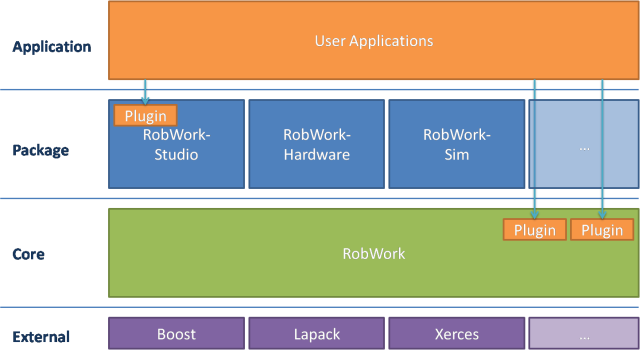
\includegraphics[scale=1]{Figures/RWOverview.png}
	\caption{Overview of the RobWork project \cite{RW_Overview}}
	\label{fig:RWOverview}
\end{figure}
\clearpage

\section{The RobWork library and its functionalities}
\label{sec:RW_lib_and_func}
This chapter is a general introduction to the RobWork library and the most commonly used data structures and functionalities within. There is a lot more to RobWork than what is in this chapter, the point of this chapter is to give a intuitive understanding of the RobWork library. More information about RobWork can be found on official homepage for the RobWork project \cite{RW_Webpage}.


\subsection{WorkCells}
A WorkCell is the basis structure in RobWork. The WorkCell can be thought of as a box containing all of the other building blocks and information needed to represent an environment (See figure~\ref{fig:WorkCellBoxExample}). The WorkCell most commonly contains Frames, Objects, Devices which are used to represent the different items in the environment. The WorkCell also contains a State Structure used to describe how the items in the environment are related. The WorkCell also contains collision information for the environment.

\begin{figure}[h]
	\centering
	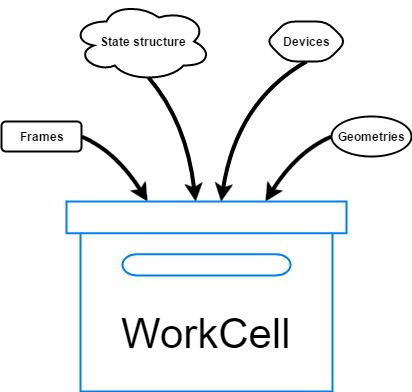
\includegraphics[scale=0.55]{Figures/WorkCellBoxExample.png}
	\caption{The WorkCell can be seen as a box containing the elements necessary to represent an environment}
	\label{fig:WorkCellBoxExample}
\end{figure}


\subsection{Frames}
One of the most common data structures from the RobWork library is a frame. A frame is the basic building block in the RobWork library, representing (in the case of RobWork) a local 3D euclidean space. In RobWork frames are built in sequence to each other to form the environment. This means that all frames have a parent and potentially children.\\

In RobWork frames come in 3 different types: fixed frames, moveable frames and joints.\\
Fixed frames are frames that have a constant transform relative to the parent frame.\\
Movable frames are frames which transform can be freely changed.\\
Joints are frames that can be assigned values for position, velocity limits and acceleration limits. This type of frame is usually used for devices. Joints can be further divided into 3 subtypes: prismatic joint, revolute joint and dependent joint.\\
Prismatic joints are joints which motion is linear along a constant direction. Thinking of a pneumatic piston can be an intuitive way of thinking about prismatic joints.\\
Revolute joints are joints which motion is based on a rotation around a single axis. Thinking of hinges can be an intuitive way of thinking about revolute frames.\\
Dependent joins refer to joints which transform depends on one or multiple other joints. Dependant joins can also be divided into 2 subtypes, dependent prismatic joints and dependent revolute joints, adding the motion specification of the prismatic joint and revolute joint previously mentioned.\\

Frames in a WorkCell are required to have a parent and are given a unique name so that no frames can be confused for another. Only one frame in the WorkCell has no parent. This frame is called WORLD and is created when the WorkCell is constructed. The WORLD frame can be seen as the global 3D euclidean space for the WorkCell.


\subsection{Objects}
Contrary to frames which represents the relationships in the environment, objects represents physical things in the scene. Also contrary to frames is that the name of an object does not have to be unique.\\

In order for objects to get a relationship to the environment it is placed in, it has to be associated to a frame. This frame is called the base frame of the object. An object can be associated to multiple frames but only have one base frame.\\

An object consists of two important elements, a geometry and a model.\\
A geometry is used to represent the actual geometry of the object. The geometry can be scaled and transformed to allow for modifications. In order to perform a transform, the geometry need a reference. This is done with having the reference be a frame, a reference frame. RobWork is capable of creating simple geometries like spheres, boxes and cylinders, however it is also possible to import complex geometries. Geometries are also being used for the collision detection provided in RobWork.\\
A model is a graphical representation of the object. Models consists of geometries, materials, colors and texture information as well. It is also possible to apply a transform to a model and get the transform of a model.\\
Usually when an object is created, a geometry is created for collision detection and a model is created to visually represent the object in a viewer(e.g. RobWorkStudio).\\

There are two types of objects in RobWork, rigid objects and deformable objects. Rigid objects are objects which  geometry does not change. Rigid objects can also posses information about inertia and mass. A deformable object however has the ability to alter its geometry via control nodes.


\subsection{Devices}
A device can be considered a description of a arbitrary device e.g. the FANUC LRM200 robotic arm (Seen on figure~\ref{fig:FANUCLRM200}). The device also contains the configurations for the device it represents. These configurations are contained in a single configuration vector, making it easy to control the device. In case of a joint device (like the FANUC LRM200), it is also possible to get and set the bounds, velocity limits and acceleration limits for the joints.\\

\begin{figure}[h]
	\centering
	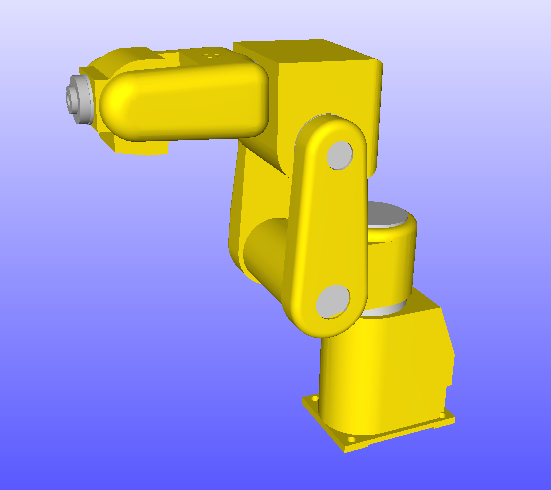
\includegraphics[scale=0.55]{Figures/FANUCLRM200.png}
	\caption{Model of a FANUC LRM200 in RobWorkStudio}
	\label{fig:FANUCLRM200}
\end{figure}

Devices can be of 3 different types: joint device, mobile device and SE3 device. Mobile devices are devices that  is differentially controlled e.g. a robot rover. Joint devices are devices that consists of moving joints much like the previously mentioned FANUC LRM200 robotic arm. SE3 devices are devices that can move in a 3D euclidean space and is not consisting of joints e.g. a drone.\\

Joint devices can be of 5 types: Serial devices, tree devices, parallel devices, composite devices and composite joint devices.\\
Serial devices are the simplest form of device since it consist of joints set in serial to each other. Many simple robotic arms like the before mentioned FANUC LRM200 are serial devices.\\
Tree devices are devices which joints follow a tree structure, meaning that a joint can have multiple children but only one parent joint. This also means that a tree device must have more than one end effectors. This type of device is typically seen in dexterous hands.\\
Parallel devices are devices that at some point in the structure, of the device, is created a circle e.g. a joint goes to two joints that then both go to the same joint. The two middle joints are said to be in parallel to each other and are called parallel legs in RobWork. Parallel legs can consist of multiple joints as well as just one.\\
Composite devices and composite joint devices are devices that are constructed from a series of other devices. The devices in the composite device may not share joints. Just like tree devices, composite devices can have multiple end effectors. However unlike the tree devices, composite devices does not require the path to the end effectors to have a common base. The difference between composite devices and composite joint device is that the devices used in a composite joint device needs to be of the joint device type, whereas in a composite device this is not a requirement.\\
Illustrations of the joint device types can be seen on figure~\ref{fig:DeviceTypes}.

\begin{figure}[h]
	\centering
	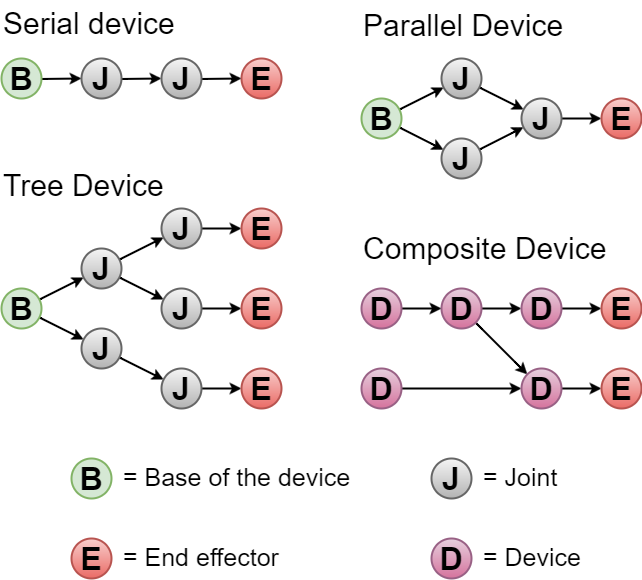
\includegraphics[scale=0.55]{Figures/DeviceTypes.png}
	\caption{The WorkCell can be seen as a box containing the elements necessary to represent an environment}
	\label{fig:DeviceTypes}
\end{figure}


\subsection{States and State Structures}
In RobWork the structure of the frames are represented through a class called State Structure. The State Structure also holds the state of all the frames in the form of a class called State. The State is a collection of the states of all the frames contained in the State Structure. This is done as a kinematic tree.


\subsection{Namespacing in RobWork}
The RobWork library is neatly divided into sections. Some of the more used sections are kinematics, models, geometry, loaders and math. When writing code using the RobWork library the namespace of the class one would want to access is the same as division of the library. As an example, accessing the the frame class from the kinematics section would be done like rw::kinematics::Frame. This makes it easier to locate the implementation of a class or fuctionality e.g. the implementation of the frame class is in the kinematics folder.\\

Most of the functionalities in RobWork are implemented as static functions. This makes coding with the RobWork library more intuitive since for some of the functionalities in RobWork it does not make sense to require an object to access the functionalities. As an example, accessing the load function of the XMLRWLoader (which loads in a XML-file describing the WorkCell) can be done simple by writing rw::loaders::XMLRWLoader::load(input for function), instead of creating a object of the XMLRWLoader and then calling load on the object.


\subsection{Typical use of RobWorkStudio and WorkCell-files}
Typically when using RobWorkStudio, the user create a WorkCell file written in XML. This file contains the necessary information for creating a WorkCell. The WorkCell file can then be loaded into RobWorkStudio by using the open button. The WorkCell file can also be loaded manually with the before mentioned XMLRWLoader returning a WorkCell object. When creating a WorkCell file it is necessary to know the tags used by RobWork. The root element in a WorkCell file is the WorkCell tag. The WorkCell tag should be written with the attribute name, giving the WorkCell a name. Inside the WorkCell tag different tags can be used to add the elements of the WorkCell. Some of the more common tags used are: frame, RPY, pos, joint, geometry tags, device tags and the include tag.\\
The frame tag is used to define a frame in the structure. The frame tag needs to be supplied with a name attribute and a type attribute defining the frame type.\\
The RPY tag is used within the frame tag to define the rotation of the frame and the pos tag is used to define the displacement. A transform can be used instead of these if the transform is available.\\
The joint tag is representing a frame of the type joint. This tag also needs a name attribute and a type attribute to define the type of joint.\\
There are also some simple geometry tags that are used for define simple geometries like a box. More complex geometries can be included via a polytype tag taking in the path for the model file.\\
Devices can be defined using different tags that define the different kind of devices in RobWork. As an example the serial device FANUC LRM200 would have a serial device tag with joint tags inside.\\
The include tag is used to include another XML file's content. This is usually used to include complex devices into an environment. This allows users to create only one description of a device and then include it whenever it is used. An example of a WorkCell described in XML can be seen in figure~\ref{fig:XMLCodeExample}.

\begin{figure}[h]
\centering
\lstset{language=XML} 
\begin{lstlisting}[frame=single]
<!-- WorkCell with the name attribute set to Scene -->
<WorkCell name="Scene"> 

<!-- New Frame called Table added to the World frame -->
  <Frame name="Table" refframe="WORLD" >
	<!-- Transform of the Table frame -->
    <RPY>0 0 0</RPY><Pos>0.2 0.2 -0.408</Pos> 
  </Frame>
  
<!-- New model named Table added to the Table Frame -->
  <Drawable name="Table" refframe="Table" >
	<!-- Transform of the model Table -->
    <RPY> 0 0 0</RPY> <Pos> 0 0 0 </Pos>
	<!-- Model information (box) of the model -->
    <Box x="0.8" y="0.8" z="0.816" />
  </Drawable>

<!-- New Frame called URMount is added to the frame Table -->
  <Frame name="URMount">
	<!-- Transform of the URMount frame -->
    <RPY>90 0 0</RPY><Pos>0 0 0</Pos> 
  </Frame>
  
<!-- Include the UR robotic arm from another xml file -->
  <Include file="../../XMLDevices/UR-6-85-5-A/UR.wc.xml" />	

</WorkCell>			 
\end{lstlisting}
\caption{Example of a WorkCell written in XML containing a UR robotic arm on a table. This example is from the examples following the the RobWork library (ModelData/XMLScenes/RobotOnTable)}
\label{fig:XMLCodeExample} 	
\end{figure}


\clearpage

\section{Qt}
%short introduction to the chapter
Qt, pronounced "cute", is an open source cross-platform framework, mostly used for GUI(graphical user interface) programming. Qt has an easy to (re)use API(application programming interface), which in return gives high developer productivity. QT is C++ class library, hence new developers using Qt should have some understanding of C++.
This chapter introduces terminologies used in Qt, and tries to give some general insight to how Qt operates and works regarding GUI development. For more information please refer to \cite{QtDocumentation}.

%Maybe something about licencing and version used.


%somewhere here should the "simple" inheritance diagram be.

\subsection{Qt Class Hierarchy and Object Model}
\label{sec:QtClassHierarchyAndObjectModel}
Qt broadly uses inheritance to create subclasses of instances in a natural way. QObject is the most basic class in Qt, see FIGURE. A lot of classes inherit from QObject, like QWidget, which is the base of all user interface objects. 
C++ offers efficient runtime for a object oriented scheme, but lacks in regard to flexibility due to the static nature of the C++ Object Model. Qt has implemented the QObject as the hearth of the Qt Object Model, which preserve the efficient runtime while also offering more flexibility for the GUI domain. The Qt Object Model is implemented with standard C++ techniques. Some of the features that the Qt Object Model adds are e.g.

\begin{itemize}
\item Inter-Object Communication called Signal and Slots in the Qt Object Model. This topic is expanded upon in section~\ref{sec:signalandslots}.
\item Object Trees which structures ownership of objects in a natural fashion. This topic is expanded upon in section~\ref{sec:qwidgets}.
\end{itemize}

\subsubsection{The Meta-Object System}
Due to the Qt Object Model the Meta-Object System was in turn created, which on the bottom line provides the Signal and Slots for inter-object communication and other features from the the QT Object Model. The Meta-Object System is based on three things:
\begin{enumerate*}[label={\alph*)},font={\color{red!50!black}\bfseries}]
\item the QObject class
\item the Q\_OBJECT macro and
\item the Meta-Object compiler(moc).
\end{enumerate*}
Each QObject or subclass of QObject has an instance of QMetaObject created to hold the meta-data information, e.g. the name of the class or the class's meta-methods(signal, slots and other member functions). The Q\_OBJECT macro helps and defines the meta data for the moc at compile time. Please refer to figure~\ref{fig:QtC++BuildProcess} to see influence of the Meta-Object System in compile time.

\begin{figure}[h]
	\centering
	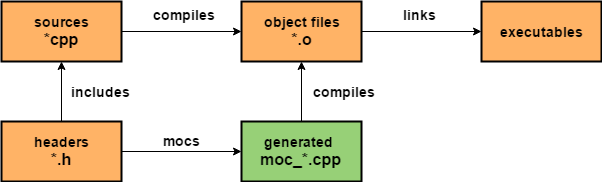
\includegraphics[scale=0.55]{Figures/QtC++BuildProcess.png}
	\caption{This figure shows how the the Meta-Object System is integrated at compile time. The yellow boxes indicate the normal C++ compiling procedure, whereas the green box is the added moc, which is compiled into the object files}
	\label{fig:QtC++BuildProcess}
\end{figure}

\subsection{QWidgets}
\label{sec:qwidgets}
QWidget is the base of all user interface objects(buttons, menus etc.). QWidget handles all events from the system the application is running on, i.e. In Qt, events are QEvent objects which is created upon outside activity (like a click on a mouse). Subclasses of QEvent involve more parameters to characterize a certain event, e.g. mousePressEvent(QMouseEvent* event). The event object is then sent to a specific QWidget object (maybe a button) and the QWidget handles the event with the according event handler.\\

As mentioned in~\ref{sec:QtClassHierarchyAndObjectModel} ownership of objects is structured in a tree, this means that a QWidget can have QWidget's within it self, see figure~\ref{fig:QWidgetExample}. A QWidget with no parent is called a top-level widget, which means the QWidget is an independent window. An instance like QWidget subclass QDialog(a pop up dialog window) is a top-level widget. QDialog can be instantiated with a parent, but the QDialog is still a top-level widget in this case, though the position of the dialog window is now centred relative to the parent.

\begin{figure}[h]
	\centering
	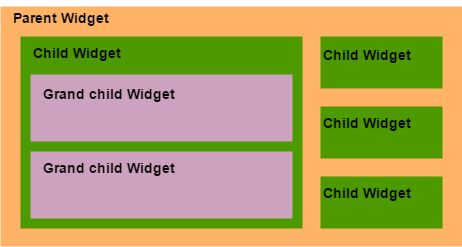
\includegraphics[scale=0.55]{Figures/QWidgetExample.png}
	\caption{Qt structures ownership of objects in a parent child relationship. The diagram shows a parent widget with various child widgets in a layout, more on layouts in section~\ref{sec:QLayout}.}
	\label{fig:QWidgetExample}
\end{figure}

When a QWidget is used as a container to hold and group children, the QWidget is called a composite widget. A parent widget is clipped to the size that it children requires, though this can be changed in the widget's size policy. 

\subsubsection{QMainWindow}
QMainWindow is a subclass of QWidget, and is very essential to a Qt GUI application, since the QMainWindow is a framework for the application user interface. As seen on figure~\ref{fig:QMainWindowExample} a QMainWindow can have a menu bar widget, toolbar bar widgets, docked widgets and a status bar widget, though a QMainWindow must have a central widget, even if that widget is only a empty placeholder. 

\begin{figure}[h]
	\centering
	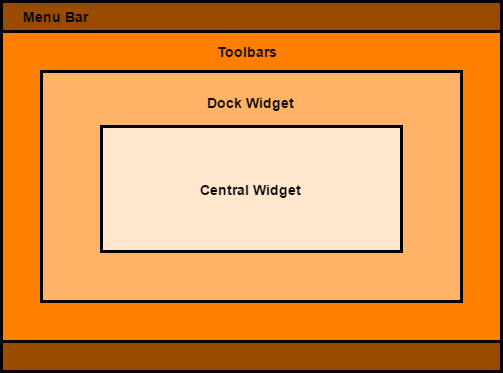
\includegraphics[scale=0.55]{Figures/QMainWindowExample.png}
	\caption{This figure shows how a QMainWindow object looks like. RWS uses QMainWindow as the main application widget.}
	\label{fig:QMainWindowExample}
\end{figure}

QMainWindow is usually a good class to use as the framework for an GUI application, though it is optional whether to use it or not. In the case of RWS, QMainWindow is used, and figure~\ref{fig:QMainWindowExample} nicely reflect the structure of RWS' GUI, where the central widget is a custom subclassed QWidget using Qt GUI modules providing classes for OpenGL integration for graphic rendering. Various plug-ins to RWS are available to be docked in the docking area, or to be top-level windows (more on plug-ins in section~\ref{sec:plugin}) and tool bars and a menu bar are present as well for use.

\subsubsection{QLayout}
\label{sec:QLayout}
QLayout is a subclass of QObject and QLayoutItem and is the base class of geometry managers. QLaoyt and it's subclasses are managers for the layout of a group of widget laid out in an application. All QWidget subclasses can use layouts to manage it's children e.g. figure~\ref{fig:QWidgetExample} uses the parent widget as composite widget with two composite children. The parent on figure~\ref{fig:QWidgetExample} use a QHBoxLayout, which lines the child widgets horizontally and makes each child fill one box. The children then has their own QVBoxLayout, which lines their children (grand children) vertically and assign each of those their own box as well. Figure~\ref{fig:QLayoutCode} shows how an implementation of five arbitrary widgets laid in the layout as in figure~\ref{fig:QWidgetExample}.

\begin{figure}[h]
\centering
\lstset{language=C++} 
\begin{lstlisting}[frame=single]  
QWidget* parent = new QWidget();  			//Parent widget
QHBoxLayout* pL = new QHBoxLayout();		//Layout of the parent widget
QWidget* cL = new QWidget(parent); 			//Left child widget
QVBoxLayout* cLL = new QHBoxLayout();		//Layout of left child widget
QWidget* cR = new QWidget(parent); 			//Right child widget
QVBoxLayout* cRL = new QHBoxLayout();		//Layout of right child widget
pL->addWidget(cR); pL->addWidget(cR);		//add children to layout
parent->setLayout(pL);						//set layout
QWidget* b1 = new QWidget(cL), b2 = new QWidget(cL), b3 = new QWidget(cR),
		 b4 = new QWidget(cR), b5 = new QWidget(cR); //create grandchildren
cLL->addWidget(b1), cLL->addWidget(b2);	//grand children added to layout
cL->setLayout(cLL);					//set layout
cRL->addWidget(b3), cRL->addWidget(b3), cRL->addWidget(b5);				 
cR->setLayout(cRL);			 
\end{lstlisting}
\caption{write stuff}
\label{fig:QLayoutCode} 	
\end{figure}


\subsection{Signal and Slots}
\label{sec:signalandslots}
Communication -> objects
Alternative to callback -> explain callback
Signal and slots -> connect() RET TO FIGURE
Signal -> 
Slot -> normal function (only special thing is it can be connected to a signal) -> found by moc
\subsubsection{Difference between events and Signal/Slots}

\subsection{Plug-in}
\label{sec:plugin}



\section{Plugin Analysis}
Gaining a better understanding of the design of the plugin based on the user needs and wants, before a development process begins. This chapter goes through the process of understanding the problem that is the basis of the plugin and help specify a generalization of how the solution should look. In the end a specified list of requirements is acquired. These requirements are used to guide the solution and in the end, test the solution.

\subsection{Using RobWorkStudio}
Since we (the authors) had never worked with RWS before. We had no personal experience regarding the problem and had to gather information about how RWS is used before implementing a solution (i.e a plug-in). The primary method to gather this information has been through interviews, to learn about the difficulties and limitations of the current solution/system.

The interviews conducted were largely semi-structured interviews, i.e. an open interview with a template for the interviewer to direct the interview in a proper direction. See appendix for the template used, however this template does not truly reflect what was learned from the interview. The reason for this type of interview, was to keep an open mind and try to get as many creative suggestions and inputs on how the interviewees uses RWS and how they alternatively would like to use it. The interviews lasted from 15 minutes to 30 minutes depending on the interviewee.

The people interviewed are as follows:

\begin{labeling}{Thomas Fridolin Iversen}
\item [Lars-Peter Ellekilde] Lektor at The Mærsk Mc-Kinney Møller Institute, SDU Robotics
\item [Thomas Nicky Thuelsen] Engineer, Research Assistant at The Mærsk Mc-Kinney Møller Institute, SDU Robotics
\item [Thomas Fridolin Iversen] Ph.d student at The Mærsk Mc-Kinney Møller Institute, SDU Robotics
\item [Michael Kjær Schmidt] Student at The Mærsk Mc-Kinney Møller Institute, SDU Robotics
\item [Kristian Møller Hansen] Student at The Mærsk Mc-Kinney Møller Institute, SDU Robotics
\end{labeling}

There were a general interest for the problem at hand, since writing XML files and adjusting a WorkCell can be a tedious process. For new users of RWS the problem was clearly recognized, since learning the syntax for the XML files can be quite daunting and slow to get started with. The potential of also being able to show something fast in RWS without having to do much work on setting anything up, was seen as a great asset.

Some of the more concrete functionalities and ideas, that was discussed in the interviews, are summarized in the following bullet points.

\begin{itemize}
\item There should be some overview of which elements the user can insert. Maybe in categories or in some other intuitive way.
\item When inserting anything, a pop-up window with adjustable parameters regarding the element, should appear, so the user can specify how the element should be inserted.
\item Insertion of a device, read from an XML file, onto another device as the end-effector should be possible.
\item Insertion of a device should snap, in a graphical drag and drop fashion, onto another device.
\item When browsing the available devices, a description box with pictures and specification about the device should be shown.
\item There should be some way to define a library of devices, which are then available to be loaded into the WorkCell.
\item Insertion of an element into the WorkCell should happen in a drag and drop fashion.
\item Static primitives and frames should be available as something to be inserted.
\item Deletion of elements in the WorkCell should be possible.
\item A undo button for the last insertion/deletion should be available for use.
\end{itemize}

\subsection{Defining use cases}
From the interviews a clearer understanding of the use of RobWorkStudio and some general pointers towards the design of the solution was established. From this some general use cases where made, describing the current use of RWS (with XML files). The use cases created were for adding a frame/geometry, adding a device and deleting an element. The use case for adding a frame/geometry can be seen on figure !!!!!.

Based on these use cases an additional set of use cases were made describing the potential use of the plugin. This set of use cases, combined with the first set of use cases, was used to verify that the creation of the plugin would actually be beneficial for the user. The use case for adding a frame/geometry for the potential use of the plugin can be seen on figure !!!!!.

\subsection{Requirement specification}
The requirements are used to specify the solution. The requirements for the project is based on the interviews and the use cases. The requirements have been divided into 2 sections, “need to have” and “nice to have”. The “need to have” requirements are requirements that needs to be fulfilled by the solution and should be verifiable , whereas the “nice to have” requirements should not necessarily be fulfilled and can be more subjective. It was decided, that devices should be described via a XML-file, as it is the standard already in use. It also makes it possible to use the parsers from RobWork to get the information from the device. It was also decided, that the ideas revolving use of the 3D view was ignored, since it would require a lot of research contra the time available to come up with a solution.\\

Need to have requirements:
\begin{enumerate}
	\item The user should be able to create fixed frames and movable frames through the plugin.
	\begin{enumerate}
		\item The user should be able to specify the parent frame for the new
		 frame.
		 \item It should be possible for the user to give the device an initial placement and rotation.
	\end{enumerate}
	\item The user should be able to create geometric primitives through the plugin.
	\begin{enumerate}
		\item The geometries are: Boxes, Planes, Spheres, Cones, Cylinders and Tubes.
		\item It should be possible for the user to give the geometries an initial placement and rotation.
	\end{enumerate}
	\item The user should be able to insert a device described by a XML-file.
	\begin{enumerate}
		\item It should be possible for the user to supply a path to a XML-file containing the description of a device.
		\item It should be possible for the user to define the parent frame of the device.
		\item It should be possible for the user to give the device an initial placement and rotation.
	\end{enumerate}
	\item It should be possible to remove frames, geometries and devices through the plugin.
\end{enumerate}

Nice to have requirements:
\begin{enumerate}
	\item The GUI of the plugin should be intuitive to use.
	\begin{enumerate}
		\item Overview of potential parent frames when inserting a new frame, device.
	\end{enumerate}
	\item The user should be able to define a library of devices for easier insertion.
	\item The user should be able to undo an action via a button or a pressing a key sequence (like ctrl + z).
\end{enumerate}

\clearpage

\section{The User Interface}
\label{sec:UserInterface}
As an introduction to the solution, this section explores the user interface of the plugin. When the plugin is loaded and opened, the user is met with figure~\ref{fig:EasyInsertDevice}. This is the Device tab of EasyInsert and from here it is possible to select a device listed and load it into the WorkCell by pressing the Load button. Upon pressing Load, the user is prompted with a dialog window where the user can specify options about the loaded device. Figure~\ref{fig:loadDialog} is the exact dialog window the user would see after selecting a device and pressing the Load button. The user can now give the device a unique name, select a frame that the device should be on and specify the configurations such as displacement and rotation. A user can now select e.g. a FANUC LRM200 robotic arm, as the one on figure~\ref{fig:FANUCLRM200}, and insert it. Afterwards the user can then select another device, let's say some kind of hand device, and now insert that device on the end frame of the fanuc. The hand device now acts as the end effector of the fanuc, which only took a few clicks to set up. 

\begin{figure}[h] % 3 figures of the tabs
        \begin{subfigure}[b]{0.32\textwidth}
                \centering
                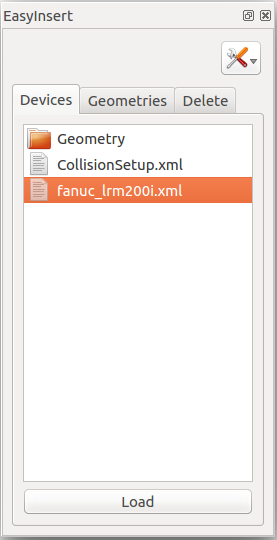
\includegraphics[width=.95\linewidth]{Figures/EasyInsertDevice.png}
  				\caption{Devices}
 				\label{fig:EasyInsertDevice}
        \end{subfigure}%
        \begin{subfigure}[b]{0.32\textwidth}
                \centering
                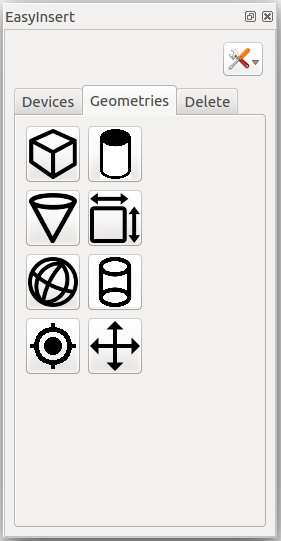
\includegraphics[width=.95\linewidth]{Figures/EasyInsertGeo.png}
  				\caption{Geometries}
  				\label{fig:EasyInsertGeo}
        \end{subfigure}%
        \begin{subfigure}[b]{0.32\textwidth}
                \centering
                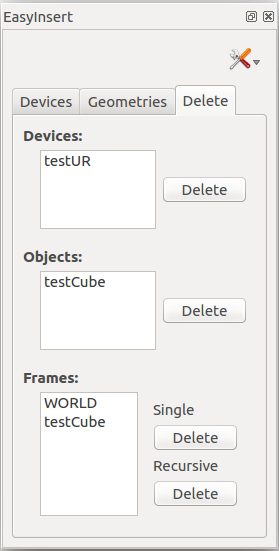
\includegraphics[width=.95\linewidth]{Figures/EasyInsertDelete.png}
  				\caption{Delete}
  				\label{fig:EasyInsertDelete}
        \end{subfigure}%
        \caption{The three tabs a user can interact with in the plugin. In Devices it is possible to select and load a device. In Geometries the user can click an icon (representing a geometry) which then prompts a dialog window with options regarding the insertion of said geometry. In Delete a user can select either a Device, Object or Frame to delete it.}\label{fig:EasyInsertTabs}
\end{figure}

It should be noted, that the first time EasyInsert is loaded and opened, the device tab shows the root content of the operating system. Thus the user needs to change the path of the list shown in the Device tab to a path containing any desired devices. In the right top corner of the plugin is a tool bar button (the only button in the tool bar so far) called settings. Clicking this button and choosing Libraries will prompt the user with the dialog window on Figure~\ref{fig:settingsDialog}. The user can here see what path is used and change it with the [...] button. The [...] button shows a new dialog window where the user can navigate his/her operating system and specify the path that should be shown in the Device tab.\\

\begin{figure}[h] % 3 figures of dialog windows
     \centering
     \begin{subfigure}[b]{0.45\textwidth}
	  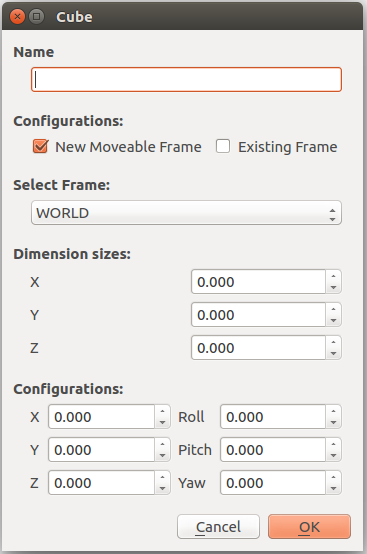
\includegraphics[scale=0.7]{Figures/EasyInsertCubeDialog.png}
       \caption{Cube insertion dialog window}\label{fig:cubeDialog}
     \end{subfigure}
     \hfill
     \begin{minipage}[b]{0.45\textwidth}
       \begin{subfigure}[b]{\linewidth}
	    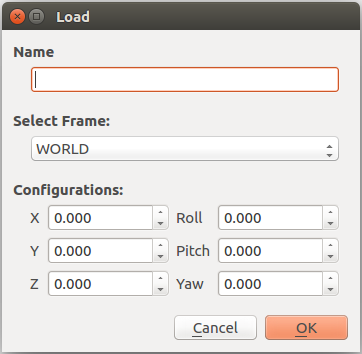
\includegraphics[scale=0.7]{Figures/EasyInsertLoadDialog.png}
         \caption{Device insertion dialog window}\label{fig:loadDialog}
       \end{subfigure}\\[\baselineskip]
       \begin{subfigure}[b]{\linewidth}
	    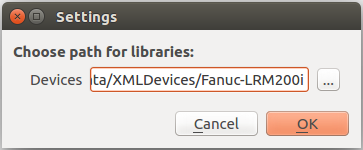
\includegraphics[scale=0.7]{Figures/settingsDialogWindow.png}
         \caption{Settings of device path dialog window}\label{fig:settingsDialog}
       \end{subfigure}
     \end{minipage}
     \caption{Three, out of many, dialog windows the user can experience and interact with when using EasyInsert.}\label{fig:EasyInsertDialogs}
\end{figure}

The Geometries tab shows a grid of icons, see figure~\ref{fig:EasyInsertGeo}. These icons represent either geometric primitives or frames that can be inserted into the WorkCell. Currently there are the following objects in the Geometries tab, from top row to bottom:
\begin{enumerate*}[font={\color{red!50!black}\bfseries}]
\item Cube.
\item Cylinder.
\item Cone.
\item Plane.
\item Sphere.
\item Tube.
\item Fixed frame.
\item Movable frame.
\end{enumerate*}
These icons are all buttons the user can click, and after a click has occurred a dialog window appears with options regarding the insertion of said geometry. When the user hovers over a button in the Geometries tab, a tool tip identifying the icon appears, telling the user what sort of object it is. Figure~\ref{fig:cubeDialog} is the dialog window prompted when clicking the cube icon, and as seen, the user can specify a name for the geometry, select a reference frame and set the displacement and rotation configurations, just like when inserting a device. Though for a geometric primitive, like the cube, the user can also specify the dimensions of the geometric figure. The user can also specify whether the primitive should create a movable frame to associate the object with, or if the user want to use an existing frame.\\

The Delete tab, as seen on figure~\ref{fig:EasyInsertDelete}, is a tab where the user can select a device, object or a frame and press either the Single Delete or Recursive Delete button to remove said item from the WorkCell. The Devices list, shown in the Delete tab, shows a device name. This means that when the user deletes a device, the frames associated with that device are now "free", i.e. the device property is deleted, but the frames and objects are still in the WorkCell. These object and frames will now show up in the Object list and the Frames list of the delete tab, and the user can now remove the frames and objects from the WorkCell. The Object list of the delete tab only deletes objects, but if the user selects a frame from the Frame list and deletes it with either the Single Delete or Recursive Delete, all objects associated with that frame will also be deleted. Single Delete will only delete the selected frame, and if that frame has children, then the user will be noticed and the deletion is cancelled. Recursive Delete deletes the frame and all children of said frame. It should be noted that there are various problems with the frame delete functionalities, certain scenarios will cause a segmentation fault (properly a rogue pointer somewhere) in the program because of different reasons. These issues will be further discussed in section~\ref{sec:eiProblems}.
\clearpage

\section{Inserting frames and geometries}
\label{sec:iframAGeom}
This section contains the description of the implementation of inserting frames and geometries. This is done trough a class called creator we made specifically for creating RobWork specific objects without a XML file description.

\subsection{General explanation of the solution}
\label{subsec:iFramesAGeomsGE}
The solution to the requirements related to insertion of frames and geometries was condensed into two parts, a user interface for the information needed (GUI) and the actions needed to insert the frames with the informations gotten from the user interface. In order to simplify the process of inserting frames and geometries, with the information given, this was separated into an extension to the RobWork library. The name chosen for this extension was creator since its focus was on creating and adding elements from the RobWork library.\\

Separating the problem into the GUI and creator have several benefits. First of all, it has the benefit of modularity. The creator is not dependant on a the GUI and is written in a way that allows use in other applications than this one.\\
Another reason is that it makes it easier to divide the task as long as the the information needed is agreed upon.

\subsection{Using the creator}
\label{subsec:iframAGeomUsing}
The creator follows the same namespacing technique as RobWork employ in order to make it more intuitive to use next to RobWork. However instead of using rw as the first namespace, ei (for EasyInsert) is used. This could be changed to rw in order make the blend perfect, however it was chosen not to in order to make the user aware that the creator is not part of the official RobWork library.\\

In the case of frames, the creator is capable of creating fixed frames and movable frames. The creator is also able to add them to a supplied WorkCell and in the case of the movable frame, give it an initial transform in the WorkCell. The fixed frame should always be supplied with a transform, since this is a criteria for the fixed frame type. 
Both functionalities returns a handle to the newly created frame which the user can user instead of being forced to search the WorkCell for a handle after creating the frame.\\

In the case of geometric primitives, the creator is capable of adding 6 different geometric primitives to a specified WorkCell: boxes, planes, spheres, cones, cylinders and tubes. No matter what geometric primitive the user wishes to create, the user needs to provide the WorkCell. The user also needs to provide a pointer to the frame they wish to include the geometric primitive to. Instead of this the user can supply the name of a parent frame for a new movable frame on which the geometric primitive is put. The user also needs to provide the necessary information in order to create the different geometric primitives. This varies between the different geometric primitives, a list of the different inputs need for the different geometric primitives can be seen on figure~\ref{fig:InputsForGeoms}. It is also possible to supply the function with a transform which then represents the local transformation of the geometric primitive in relation to the frame on which it has been included.\\

\begin{figure}[h]
	\centering
	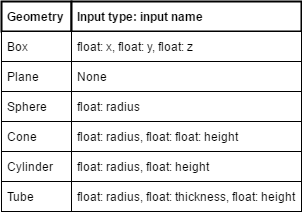
\includegraphics[scale=0.55]{Figures/InputsForGeoms.png}
	\caption{Table of geometric specific inputs for the individual geometric primitives}
	\label{fig:InputsForGeoms}
\end{figure}

Since a lot of transformations are used in the creator it was decided also to create a function to easily create transform objects from R,P,Y and x,y,z values. The function, called getTransform3D, takes in these values and returns a Transform3D object.\\

An example of adding a sphere to a new WorkCell can be seen on figure~\ref{fig:CodeExampleAddSphere}.

\begin{figure}[h]
	\centering
	\lstset{language=C++} 
	\begin{lstlisting}[frame=single]
	// Create new wc
	WorkCell::Ptr dummy = ownedPtr(new WorkCell("wc"));
	 
	// Radius of 10 cm
	float radius = 0.1;
	
	// Displacement of 10 cm in x, y and z
	Transform3D<double> transform = getTransform3D(0.1, 0.1, 0.1, 0, 0, 0); 
	
	// Adding sphere to WorkCell
	ei::creator::addSphere( "testSphere", // Name of Sphere
							"WORLD", // Name of parent frame
							wc, // Pointer to WorkCell
							radius, // Radius of Sphere
							transform); // Transform of Sphere
	 
	\end{lstlisting}
	\caption{Code example of adding a sphere to a new WorkCell. The sphere has a radius of 10 cm and a displacement of 10 cm in x, y and z in relation to the frame on which it is set. The sphere is added to a new movable frame with the parent set to the WORLD frame.}
	\label{fig:CodeExampleAddSphere}
\end{figure}

\subsection{Implementation of the creator}
The creator was implemented with the purpose of using the most upper layers of the RobWork libraries functions to solve as much of the problem as possible. This was done since in RobWork it is possible to access lower levels of the library which makes the RobWork library way more flexible. An example of this could be when working with the frames of a WorkCell the upper layer way of doing it would be accessing the frames through the WorkCell's own functionality for getting frames, whereas the lower layer of doing it would be to access the state structure in the WorkCell and through it access the frames. The other reasoning for using upper layers is that it is usually simpler code, meaning there is less mistakes to make and the mistakes made are easier to find.\\

The implementation of the getTransform3D function is rather simple since it utilises some conversions in the RobWork library. The inputs for the function are 6 doubles representing the x, y, z values, which is the displacement, and the R, P, Y values representing the rotation. In order to create a Transform3D object, a vector representing the displacement and a matrix representing the rotation is needed. The displacement vector is easy to create since it is just a vector containing the x, y, z values directly from the input. The rotation matrix however is more difficult to get since the input for the rotation is represented in R, P, Y values. The R, P, Y values needs to be converted to a rotation matrix. Instead of doing the calculations manually, RobWork, albeit a little hidden, can do this for us through the RPY class from the math namespace. First an RPY object is created with the values from the input. Then the member function toRotation3D from the RPY class is called returning the rotation matrix of the given R, P, Y values. The displacement vector and rotation matrix is then used to create a Transform3D object that is returned to the user. It would be possible to just implement the same functionality that the toRotation3D RPY class, eliminating the creation of an RPY object. This would increase the computation speed, but not significantly unless the function is used a lot.

\subsubsection{Implementation of creating and adding frames}
There are a total of 4 functions in the creator that are related to creating and adding frames to a WorkCell. The first 2, one for each type of frame, are functions related to creating frames. The implementation of creating frames in the creator is rather simple, since the process of creating frames in RobWork is simple in itself. The 2 functions are called createFixedFrame(...) and createMovableFrame(...). The createFixedFrame(...) function take the name of the frame and a transform as input, whereas the createMovableFrame(...) only takes the name as input. The functions simply call the constructor for the given frame with the provided parameters. The reasoning behind having these rather simple functionalities is in the context that the creator should be consistent in the functionality it embodies. Another good reason was that this was some of the first functionalities implemented for the creator. At the time the idea was that there would also be a function, atleast for the fixed frame, that took in the x, y, z and R, P, Y values instead of a transform. The function would then calculate the transform by itself and use this transform when creating the frame. This was however deemed unnecessary to implement when the getTransform3D(...) function was implemented.\\

The last 2 functions, again one for each type of frame, are functions that are capable of creating and adding a frame to a specific WorkCell. The two functions are called addFixedFrame(...) and addMovableFrame(...). Both of the functions take in a WorkCell, a name, a name of a parent frame and a transform. These functions eliminates the need for the user to understand how to create a frame and how to add the frame to the WorkCell. Even though one could say that this is rather simple process to learn, using the creator simplifies the process significantly. This comes at the cost of flexibility since the user is now locked to the implementation of the functions. However it was estimated that in many cases the functionality implemented in the creator could be used. Figure~\ref{fig:CodeExampleAddFrameDifference} showcases the standard way of creating a frame and the adding it to a WorkCell, versus using the creator.

\begin{figure}[h]
	\centering
	\lstset{language=C++} 
	\begin{lstlisting}[frame=single]

	string name = "test"; // Name of frame
	string parent = "WORLD"; // Name of parent frame
	Transform3D<double> transform =  // Transform used
	ei::creator::getTransform3D(1, 1, 1, 1, 1, 1);
	WorkCell::Ptr wc; // WorkCell

	/// The standard way of adding a frame ///
	
	// Create new movable frame object and cast to frame
	MovableFrame* mframe = new rw::kinematics::MovableFrame(name);
    Frame* frame = dynamic_cast<rw::kinematics::Frame*>(mframe);
    
    // Find the parent frame in wc
    Frame* parentFrame = wc->findFrame(parent);
	
	// Test for eligible parent
	if(parentFrame != NULL) {
	
		// Add the frame to the wc
        wc->addFrame(frame, parentFrame);
		
		// Get state of wc
		State state = wc->getDefaultState();
		
		// Set transform of the movable frame in the wc
		mframe->setTransform(transform, state);
		
		// Upgrade state and update state
		state = wc->getStateStructure()->upgradeState(state); 
		wc->getStateStructure()->setDefaultState(state); 
    }
	
	
	/// Using the creator ///
	ei::creator::addMovableFrame(wc, name, parent, transform);

	\end{lstlisting}
	\caption{Code example of the standard way of adding a movable frame with a transform and the same process using the creator}
	\label{fig:CodeExampleAddFrameDifference}
\end{figure}

\subsubsection{Implementation of creating geometries}
Since in RobWork a geometric primitive, like a box, is called an object, a way to create a object that contains the information to represent the geometric primitive is needed. Getting inspiration from the implementation of the RWXMLLoader (See section~\ref{subsec:XMLRWLoader}) in RobWork, it was chosen to use the same factory approach as the loader. This means that when creating the geometry part of the object, the GeometryFactory from the loaders part of RobWork is used. When the model part of the object is created the Model3DFactory is used, again from the loaders part of RobWork. All of this is neatly put into 3 functions, addObject(...), createGeom(...) and createModel(...).\\

In order to understand process of adding e.g. a box it is easiest to start from the bottom with what the factories need in order to produce the geometry and the model. From the GeometryFactory a function called load(...) is used. This function takes in a string containing the information about the geometry it needs to produce and a bool that signifies whether or not the user wishes to use cached geometries. As an example, the syntax for the string when creating a box is "\#Box dx dy dz", where dx, dy and dz are the dimensions of the box. The syntaxes for the rest of the geometries can be seen on figure~\ref{fig:SyntaxTable}. The function create createGeom(...) uses the GeometryFactory to create a geometry and return it.\\

\begin{figure}[h]
\centering
\begin{tabular}{|l|l|l|}
\hline
Geometry & Syntax                           & Explanation of parametres                                                                                                                    \\ \hline
Box      & "\#Box dx dy dz"                 & The dx, dy and dz are the dimensions of the box                                                                                              \\ \hline
Plane    & "\#Plane"                        & Planes need no parameters                                                                                                                    \\ \hline
Sphere   & "\#Sphere radius"                & The radius is the radius of the sphere                                                                                                       \\ \hline
Cone     & "\#Cone radius height"           & The radius is the radius of the cone and the height is the height of the cone                                                                \\ \hline
Cylinder & "\#Cylinder radius height level" & The radius is the radius of the cylinder, the height is the height of the cylinder and the level is the discretization level of the cylinder \\ \hline
Tube     & "\#Tube radius height level"     & The radius is the radius of the tube, the height is the height of the tube and the level is the discretization level of the tube             \\ \hline
\end{tabular}
\caption{Table showing the syntaxes for the different geometric primitives}
\label{fig:SyntaxTable}
\end{figure}

From the Model3DFactory a function called getModel(...) is used. This function takes in a string that either describes a geometry in the same syntax as the GeometryFactory or a file name. It also takes in a string representing the name of the model. It is rather beneficial that the input for describing the geometry is the same for both the GeometryFactory and the Model3Dfactory since it makes it simpler to implement. The function createModel(...) uses the model3Dfactory to create a model and return it. The function addObject(...) uses both the createGoem(...) and the createModel(...) functions when constructing the object.\\

The addObject(...) function now needs to be interfaced to the individual geometric primitives. It is also known that the addObject(...) needs to be supplied a string describing the geometry. To do this a series of easy to use functions related to the geometric primitives were created. An example of one of these is the addSphere(...) which takes in the necessary information to describe a sphere (the radius) and then creates the appropriate string for the factories. It then calls the addObject(...) function with this string, and other relevant information, which creates and adds the object to the WorkCell. An example of the function flow, using addSphere(...), can be seen on figure~\ref{fig:CreatorFlow}.

\begin{figure}[h]
	\centering
	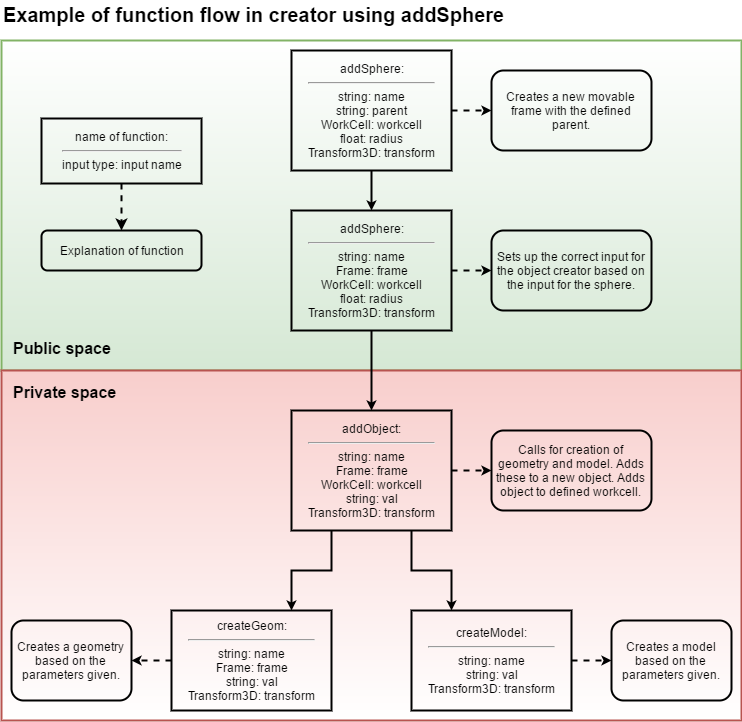
\includegraphics[scale=0.55]{Figures/CreatorFlow.png}
	\caption{Function flow of the creator using addSphere(...) as example}
	\label{fig:CreatorFlow}
\end{figure}

\subsection{The future of the creator}
Most of the functionalities that where implemented with the purpose to fulfil the requirements of the solution. The possibilities for the creator is however almost limitless. This is mostly due to the fact that the creator is written like a library extension to the RobWork library. One of the more immediate expansions to the creator that could be made, would be to extend the geometric primitive related functions with the possibility to only create the geometry or model when creating the object. This extension would make it possible to create visible objects with no collision or invisible objects with collision. Another good addition would be to create a functionality capable of loading geometries from a geometry file. This is already possible in RobWork, so it would make sense to also simplify this process in the creator.
\clearpage

\section{Inserting devices}
This section contains the description of the solution regarding adding devices to a WorkCell. The solution was heavily inspired by the XMLRWLoader from the loaders section of the RobWork library. The solution was put in a class called loader.

\subsection{General explanation of the solution}
The solution for the requirements related to insertion of devices (See need to have requirement 3) was, just like with inserting frames and geometries, divided into two parts. The first part is the interface to the user required for the user to be able to supply the necessary information needed. The second part is the process of creating and inserting the device defined by the user. The reason for this separation is the same as the one given in inserting frames and geometries section (\ref{subsec:iFramesAGeomsGE} General explanation of the solution).

\subsection{Using the loader}
The loader contains two functionalities the user should be aware of. The first functionality is a function called add. This functions adds the device described in a XML file to a given WorkCell. The function add takes in a string representing the path to the, the WorkCell which the information should be added to, a string representing the custom name of the device and a string containing the name of the frame on which the device should be placed. The user can also supply a transform which is applied to the base frame of the device, giving it an initial placement. The transform can be supplied in two different ways, the user can supply the function with a transform object or the x, y, z and R, P, Y values.\\

The loader also contains the functionality to load a WorkCell from an XML-file, just like the XMLRWLoader. This functionality was made solely to give the loader more consistency in its functionalities.\\

An example of using the loader can be seen on figure !!!!!.


\subsection{Understanding the XMLRWLoader}
In order to understand what it takes to load information from an XML-file into the format used in RobWork, it is worth the time to study the XMLRWLoader. Another good reason to study the XMLRWLoader is that it solves a problem very similar to the problem of interest in this chapter. There are only two differences, the XMLRWLoader loads not only devices and it creates a new WorkCell to put the items in.\\

The function of interest from the XMLRWLoader is the loadWorkcell function. This function takes in a single input which is a string containing the path to the XML file describing the WorkCell.\\
A good place to start is to analyse the flow that the loadWorkCell function have. The function can be seen as a sequence of actions:

\begin{enumerate}
	\item Parse the XML file using parseWorkCell from XMLRWParser contained in the loaders section. This takes in the provided path.
	\begin{enumerate}
		\item The information is parsed into a struct called DummyWorkCell that arranges the information neatly for when it should be used.
	\end{enumerate}
	\item Do sanity check on all the frames
	\begin{enumerate}
		\item Each frame needs to have a valid parent frame
	\end{enumerate}
	\item Create a new WorkCell object
	\item Create and add all the frames, defined in the DummyWorkCell, to the WorkCell
	\item Add all frame properties to the WorkCell
	\item Create all devices defined in the DummyWorkCell
	\item Create and add models, belonging to the added frames, to the WorkCell
	\item Create and add all DAF (dynamically attachable) frames to the WorkCell
	\item Create and add collision models to the WorkCell
	\item Initialize state with initial actions
	\item Add devices to the WorkCell
	\item Add objects to the scene
	\item create and add collision and proximity setup from corresponding files
	\begin{enumerate}
		\item This only applies if the files are defined in the XML file
	\end{enumerate}
	\item Add name of the WorkCell XML file and the path to the property map of the WorkCell
	\item Return the WorkCell
\end{enumerate}

It should be advised that this sequence is a intuitive understanding of the loadWorkCell function. The function does much more than this, however this is the bread and butter of the function. A more in depth illustration of how the XMLRWLoader functions can be seen on the flowchart contained in figure !!!!!.

\subsection{Implementation of the loader}
The implementation of the loader can be explained in the different capabilities that were added as time went on. The first capability of the loader was to add a device to the WorkCell. The second capability was to be able to give the device a name. The third capability was to be able to apply a transform to the device. The last capability added was the ability to define the parent frame of the device. After all of these capabilities were implemented, the loader now complies with requirements for inserting a device (See need to have requirement 3).

\subsubsection{Adding a device to a WorkCell}


\subsubsection{Custom naming the device}


\subsubsection{Adding a transform to the device}


\subsubsection{Defining the parent for the device}



In the case that the x, y, z and R, P, Y values are supplied, the loader calculates the transform from these values using the 

\subsection{The future of the loader}
\clearpage

\section{The Plug-In}
Introduction to the chapter.
Something about we first explore the user interface of the plugin, and then we look into the elements consisting within the user interface.

	What elements are there in this chapter?	
		User Interface
			All teh stuff the user can do in this plugin with pictures.	
		EasyInsert
			plug-in specific elements for RWS and how they are used.
			.ui was not used, why?
		Dialogs
		EasyInsert Construction - Bringing it all together.	
		Settings			
		Device tab
			mention something in the introduction about how the tabs will be gone through
		Geo tab
		Delete tab
		

\subsection{User Interface}
\label{sec:UserInterface}
This section explores the user interface of the plugin. When the plugin is loaded and opened, the user is met with figure~\ref{fig:EasyInsertDevice}. This is the Device tab of EasyInsert and from here it is possible to select a device listed and load it into the WorkCell by pressing the Load button. Upon pressing Load, the user is prompted with a dialog window where the user can specify options about the loaded device. Figure~\ref{fig:loadDialog} is the exact dialog window the user would see after selecting a device and pressing the load button. The user can now give the device a unique name, select a frame that the device should be on and specify the configurations such as displacement and rotation. A user can now select e.g. a fanuc robot arm, as the one on figure~\ref{fig:FANUCLRM200}, and insert it. Afterwards the user can then select another device, let's say some kind of hand device, and now insert that device on the end frame of the fanuc. The hand device now acts as the end effector of the fanuc, which only took a few clicks to set up. 

\begin{figure}[h] % 3 figures of the tabs
        \begin{subfigure}[b]{0.32\textwidth}
                \centering
                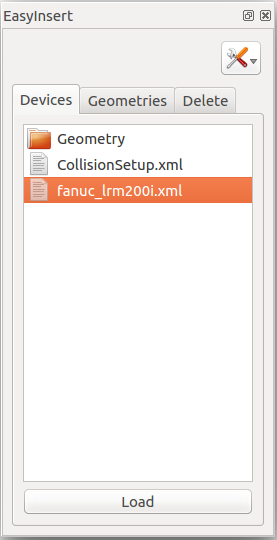
\includegraphics[width=.95\linewidth]{Figures/EasyInsertDevice.png}
  				\caption{Devices}
 				\label{fig:EasyInsertDevice}
        \end{subfigure}%
        \begin{subfigure}[b]{0.32\textwidth}
                \centering
                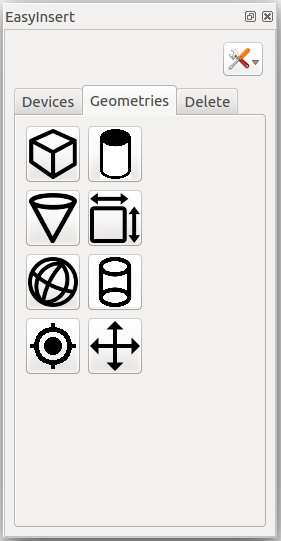
\includegraphics[width=.95\linewidth]{Figures/EasyInsertGeo.png}
  				\caption{Geometries}
  				\label{fig:EasyInsertGeo}
        \end{subfigure}%
        \begin{subfigure}[b]{0.32\textwidth}
                \centering
                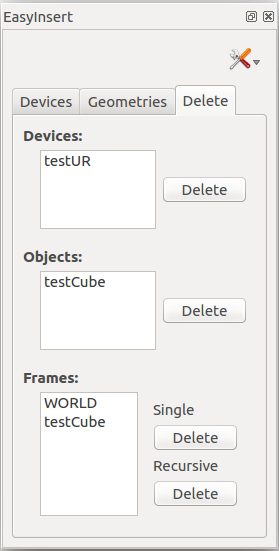
\includegraphics[width=.95\linewidth]{Figures/EasyInsertDelete.png}
  				\caption{Delete}
  				\label{fig:EasyInsertDelete}
        \end{subfigure}%
        \caption{The three tabs a user can interact with in the plugin. In Devices it is possible to select and load a device. In Geometries the user can click an icon (representing a geometry) which then prompts a dialog window with options regarding the insertion of said geometry. In Delete a user can select either a Device, Object or Frame to delete it.}\label{fig:EasyInsertTabs}
\end{figure}

It should be noted, that the first time EasyInsert is loaded and opened, the device tab shows the root content of the operating system. Thus the user needs to change the path of the list shown in the Device tab to a path containing any desired devices. In the right top corner of the plugin is a tool bar button (the only button in the tool bar so far) called settings. Clicking this button and choosing Libraries will prompt the user with the dialog window on Figure~\ref{fig:settingsDialog}. The user can here see what path is used and change it with the [...] button. The [...] button shows a new dialog window where the user can navigate his/her OS and specify the path that should be shown in the device tab.\\

\begin{figure}[h] % 3 figures of dialog windows
     \centering
     \begin{subfigure}[b]{0.45\textwidth}
	  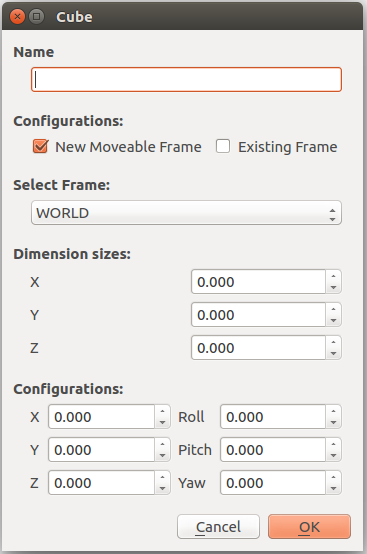
\includegraphics[scale=0.7]{Figures/EasyInsertCubeDialog.png}
       \caption{Cube insertion dialog window}\label{fig:cubeDialog}
     \end{subfigure}
     \hfill
     \begin{minipage}[b]{0.45\textwidth}
       \begin{subfigure}[b]{\linewidth}
	    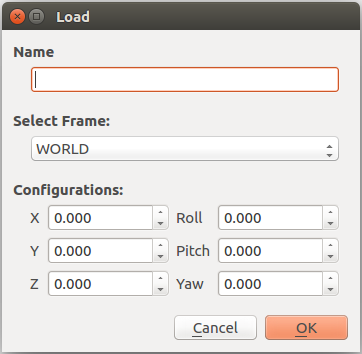
\includegraphics[scale=0.7]{Figures/EasyInsertLoadDialog.png}
         \caption{Device insertion dialog window}\label{fig:loadDialog}
       \end{subfigure}\\[\baselineskip]
       \begin{subfigure}[b]{\linewidth}
	    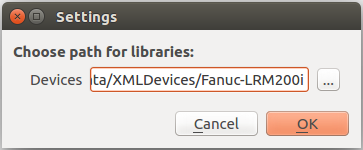
\includegraphics[scale=0.7]{Figures/settingsDialogWindow.png}
         \caption{Settings of device path dialog window}\label{fig:settingsDialog}
       \end{subfigure}
     \end{minipage}
     \caption{Three, out of many, dialog windows the user can experience and interact with when using EasyInsert.}\label{fig:EasyInsertDialogs}
\end{figure}

The Geometries tab shows a grid of icons, see figure~\ref{fig:EasyInsertGeo}. These icons represent either geometric primitives or frames that can be inserted into the WorkCell. Currently there are the following objects in the geometric tab, from top row to bottom:
\begin{enumerate*}[font={\color{red!50!black}\bfseries}]
\item Cube.
\item Cylinder.
\item Cone.
\item Plane.
\item Sphere.
\item Tube.
\item Fixed frame.
\item Movable frame.
\end{enumerate*}
These icons are all buttons the user can click, and after a click has occurred a dialog window appears with options regarding the insertion of said geometry. When the user hovers over a button, a small box identifying the icon appears, telling the user what sort of object it is. Figure~\ref{fig:cubeDialog} is the dialog window prompted when clicking the cube icon, and as seen, the user can specify a name for the geometry, select a reference frame and set the displacement and rotation configurations, just like when inserting a device. Though for a geometric primitive, like the cube, the user can also specify the dimensions of the geometric figure. The user can also specify whether the primitive should create a movable frame to associate the object with, or if the user want to use an existing frame.\\

The delete tab, as seen on figure~\ref{fig:EasyInsertDelete}, is a tab where the user can select a device, object or a frame and press the Delete button to remove said item from the WorkCell. The Devices list, shown in the delete tab, shows a device name. This means that when the user deletes a device, the frames associated with that device are now "free", i.e. the device property is deleted, but the frames and objects are still in the WorkCell. These object and frames will now show up in the Object list and the Frames list of the delete tab, and the user can now remove the frames and objects from the WorkCell. The Object list of the delete tab only deletes objects, but if the user selects a frame from the Frame list and deletes it, all objects associated with that frame will also be deleted. Furthermore, if the user selects a frame from the Frames list and deletes it, all children of children of said frame will also be deleted. It should be noted, that the Frames list of the delete tab does not update properly because of an internal bug in RWS, this means that when the user deletes a frame, the frame will still appear in the list, but if the user looks in the TreeView plugin, or searches the WorkCell, the user will notice that the frame has actually been deleted. The user is then able to delete a frame twice, which will cause a segmentation error and crash RWS. This is a critical error, but it has not been solved because solving this error is out of the scope of the project.



\subsection{Dialog Windows}
\label{sec:DialogWindows}
The dialog window is the main communication with the user in this plugin. Dialog windows are top-level windows, and they provide the user with either information, or they allow the users to select options to perform a command or task. This section will show how dialog windows has been handled in the plugin.\\

The dialogs of EasyInsert has been implemented in it's own class dialog.hpp, i.e. a subclass of QDialog, see figure~\ref{fig:subClassQWidget} for an example of a Qt subclass. This was done to keep it independent and self-contained from the rest of the plug-in. The constructor for the dialog class is very simple, see figure~\ref{fig:dialogConstructor}. A constructor with no WorkCell parameter is also available and passing a parent is optional, though a name must always be given to the constructor. 

\begin{figure}[h] % Code of dialog constructor
\centering
\lstset{language=C++} 
\begin{lstlisting}[frame=single]  
dialog::dialog(rw::models::WorkCell::Ptr wc, QString dialog, QWidget *parent)
    : QDialog(parent)
{
    _workCell = wc;
    mainLayout = new QVBoxLayout();
    setWindowTitle(dialog);
}			 
\end{lstlisting}
\caption{The dialog class constructor. A WorkCell pointer to a RW instance is passed along as a parameter. The QString parameter is the name of the dialog box and the QWidget is a pointer to the parent widget }
\label{fig:dialogConstructor} 	
\end{figure}

The dialog class is fairly simple to use and extend. A dialog is made of blocks in a vertical layout of QWidget's, i.e. a dialog instance is a composite widget containing composite widgets. Figure~\ref{fig:dialogWindowExample} shows a dialog window with four blocks initialised.

\begin{figure}[h]
	\centering
	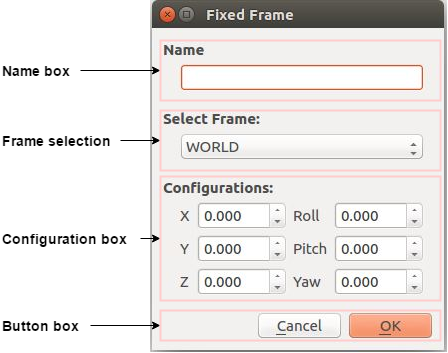
\includegraphics[scale=0.55]{Figures/dialogclassblocks.png}
	\caption{This figure shows a dialog window of adding a fixed frame to a WorkCell containing various widgets relevant to the action. }
	\label{fig:dialogWindowExample}
\end{figure}

All the blocks used to create all the dialog windows in the plug-in are shown in figure~\ref{fig:dialogBlocks}. These blocks are just member functions of the dialog class which returns a composite widget. So to create a dialog window as shown on figure~\ref{fig:dialogWindowExample}, a dialog instance should be constructed (in this case with a WorkCell pointer) and then simply adding the blocks to the dialog with the utility member function addToDialog(). See figure~\ref{fig:dialogWindowCode} which shows a code example on how to use the dialog class to construct the dialog window as shown on figure~\ref{fig:dialogWindowExample}. Since the dialog class is a subclass of QDialog, the position of the dialog window (opposed to a normal QDialog object) is always centred to the main application (RWS), even though a parent is passed as a parameter.

\begin{figure}[h] % code of adding stuff to a dialog
\centering
\lstset{language=C++} 
\begin{lstlisting}[frame=single]  
QString st = "Fixed Frame"; //Name of the dialog window
rw::models::WorkCell::Ptr wc = getRobWorkStudio()->getWorkCell(); //WorkCell
dialog* geoDialog = new dialog(wc,st,this); //Create the dialog window
geoDialog->addToDialog(geoDialog->createNameBox()); //Adding something
geoDialog->addToDialog(geoDialog->createFrameSelection());
geoDialog->addToDialog(geoDialog->createConfigurationBox());
geoDialog->addToDialog(geoDialog->createButtonBox());	
geoDialog->exec(); //execute/open dialog window	 
\end{lstlisting}
\caption{A sample code to illustrate how to construct the dialog window from figure~\ref{fig:dialogWindowExample}.}
\label{fig:dialogWindowCode} 	
\end{figure}

exec(), seen on figure~\ref{fig:dialogWindowCode} line 8, is an inherited public slot that executes/shows the dialog window. The dialog shown is in modal mode, meaning the window denies all user actions on any other widgets in the application. The function returns a DialogCode containing the information about whether the dialog window was accepted or rejected. The accepted or rejected information is determined by the user input to the createButtonBox() function block, since the OK button emits a accepted() signal to the accept() slot of the dialog object when pressed. Likewise the Cancel emits a rejected() signal to the reject() slot of the dialog object, though a rejected() signal is also emitted when the user presses ESC on the keyboard or the x(close) button of the dialog window. 

So when a dialog window has been created and used by a user, then some functionality should be executed based on the inputs given to the dialog. That means when the function exec() returns, we need to know whether the user accepted or rejected the dialog window (pressed OK or Cancel). This is done with the inherited public function result(). The function result() returns QDialog::Accepted when the dialog was accepted and QDialog::Rejected when it was rejected (QDialog::Accepted and QDialog::Rejected are both just normal enumerators, i.e. 1 and 0). 

\begin{figure}[h] % code of what to do after exec
\centering
\lstset{language=C++} 
\begin{lstlisting}[frame=single]  
geoDialog->exec();
if(geoDialog->result() == QDialog::Accepted) //Check the result
{
	std::string name = geoDialog->getNameBox(); //Get the name input
	std::string frame = geoDialog->getFrameSelection(); //Get frame selc
											 
		/*	Do something with the information    */ 
		
}
delete geoDialog; //Delete the dialog object when done using it
\end{lstlisting}
\caption{A sample code illustrating what to do after the exec()function returns.}
\label{fig:dialogAcceptedRejectedCode} 	
\end{figure}

As seen on figure~\ref{fig:dialogAcceptedRejectedCode}, after the exec() function returns, we simply check whether the result was QDialog::Accepted or not. If the result is accepted, then something should be done with the inputs given to the dialog window. We access these input via self explanatory public get-functions, e.g. the NameBox contains the name input (as seen on figure~\ref{fig:dialogAcceptedRejectedCode} line 4). After we have collected all the information we wanted out of the dialog window, then we can proceed to do something with the information, like e.g. the insertion of a frame. When we are done with the dialog window it should be deleted, because the dialog object is still alive until the parent is dead (in this case the plugin). If we do not delete the dialog object the dialog objects, created in the lifetime of the plugin, will just waste space in memory. 

It would to much time to inspect all of the function blocks on figure~\ref{fig:dialogBlocks}. Therefore only one function block, namely createNameBox() figure~\ref{fig:dialogCreateNameBoxCode} will be inspected. All the function blocks has a similar structure.

\begin{figure}[h] % code example of createNameBox
\centering
\lstset{language=C++} 
\begin{lstlisting}[frame=single]  
QWidget* dialog::createNameBox() {
    QGroupBox* nameBox = new QGroupBox(tr("Name")); //The nameBox widget
    QHBoxLayout *layout = new QHBoxLayout; //layout for the nameBox
    nameLine = new QLineEdit(); //The line edit the user can type the name
    layout->addWidget(nameLine); //Add the line edit to the layout
    nameBox->setLayout(layout); //Set the layout to the namebox
    return nameBox; //Return the nameBox
}
\end{lstlisting}
\caption{This figure shows the pulic function createNameBox() from the dialog class. The function is used to add a name line edit to dialog windows.}
\label{fig:dialogCreateNameBoxCode} 	
\end{figure}

The general procedure in the function blocks, as seen on figure~\ref{fig:dialogCreateNameBoxCode}, is to first create the composite widget. This widget, in the case of createNameBox, is a QGroupBox widget. QGroupBox is a widget that is mainly used as a composite widget. The QGroupBox provides a box to group widgets in, a frame if wanted and a title. As seen on figure~\ref{fig:dialogCreateNameBoxCode} line 2, the title is set upon construction with the string "Name". The tr() function is for translation purposes \cite{QtDocumentationTr}.
After the composite widget has been created, the layout for the parent widget has to be chosen and the child widget(s), in this case a QLineEdit(), has to be created. QLineEdit() is a simple line where text can be typed and edited in. When all the child widgets has been created, they need to be added to the layout of the parent. Lastly the layout is set to the parent and the parent is then returned. It should be noted that when the QLineEdit() was created, figure~\ref{fig:dialogCreateNameBoxCode} line 4, no parent was defined, i.e. it is actually not a child widget but a top-level widget. This is fine though, because when a top-level widget is added to a layout of another widget, that widget automatically takes responsibility as a parent and the top-level widget is now a child of that widget.

\begin{figure}[h] % table of function blocks
\centering
\begin{center}
  \begin{tabular}{ | p{6cm} | p{7cm} |}
    \hline
    \textbf{Function blocks} 	   &   \textbf{Description}  \\ \hline
    createButtonBox()			   &   The Cancel and OK buttons. This block is used in all the dialog windows.   		\\ \hline
    createNameBox() 			   &   A line edit to specify a name.   		\\ \hline
    createCheckFramesBox()		   &   Two exclusive check boxes, i.e. only one of the boxes can be checked at a time.		\\ \hline
    createConfigurationBox() 	   &   The different configurations available to adjust regarding displacement and rotation of the inserted element. 		\\ \hline
	createConfigurationBoxCube()   &   A cube specific configuration option, i.e. the dimensions of the cube.  	\\ \hline	    
	createConfigurationBoxSphere() &   A sphere specific configuration option, i.e. the dimensions of the sphere. 	\\ \hline	
	createConfigurationBoxCone()   &   A cone specific configuration option, i.e. the dimensions of the cone.  	\\ \hline	
    createConfigurationBoxTube()   &   A tube specific configuration option, i.e. the dimensions of the tube.  	\\ \hline	
	createLibSettingsBox(PropertyMap *map)		   &   This block is used to edit the settings of the device library.    	\\ \hline	 
	createFrameSelection()		   &   A way to select a parent frame for the inserted element. Default is the WORLD frame.		\\
    \hline
  \end{tabular}
\end{center}
\caption{This table summarizes all the different dialog function blocks used to construct the dialog windows in the plug-in.}
\label{fig:dialogBlocks} 
\end{figure}


Something about what could be worked on in regard to this class. Like constructors for a generic dialog window, mainlayout in a grid instead and extended adddialog functionality.
Is this something that should be in this chapter?


\subsection{EasyInsert Implementation}
This chapter will go through how EasyInsert achieved the functionalities and interfaces mentioned in section~\ref{sec:UserInterface} with the help from the dialog, creator and loader classes. 

On figure~\ref{fig:eiClass} the constructor for the plugin is seen. Before creating the widgets making up the plugin, all settings are set up with the setupSettings() function on line 4 (discussed in section~\ref{sec:Settings}). The parent widget of the plugin is then created which is a QScrollArea. A QScrollArea widget provides a scrolling view onto another widget (the child). The QScrollArea widget is created on line 5 and the widget is then set to be resizeable. When a QScrollArea is set to be resizeable, the child widget of the QScrollArea will automatically be resized so to either avoid scroll bars (decrease size of child) or utilize extra space (increase size of child). It should be noted that when QScrollArea has a composite child with a layout, the size policy of that layout will determine the size (or resize) of the widget. The composite child is created on line 7 and then a vertical layout is created. QToolbar is then created on line 9 using the createToolBar() function (discussed in section~\ref{sec:ToolBar}), the tool bar is then added to they layout and it is right aligned. On line 12 the QTabWidget is created, a QTabWidget is a widget with stacked tabs of widgets, where the user can select a tab and see the widget associated with that tab. To create a tab, a QWidget needs to be passed to the addTab function and a name can be given as well. On line 13 to 15 all the tabs are created with the help of createDevTab() (section~\ref{sec:DeviceTab}), createGeoTab() (section~\ref{sec:GeoTab}) and createDeleteTab() (section~\ref{sec:DelTab}) which all returns a QWidget. The QTabWidget is then added to the layout and set to the composite child which in turn is set to the QScrollArea widget and finally the QScrollArea widget is set to the QDockWidget of RWS. 

\begin{figure}[h] % Code of ei constructor
\centering
\lstset{language=C++} 
\begin{lstlisting}[frame=single]  
EasyInsert::EasyInsert():
    RobWorkStudioPlugin("EasyInsert", QIcon(":/pa_icon.png"))
{
    setupSettings();
    QScrollArea *widg = new QScrollArea(this);
	widg->setWidgetResizable(true);
	QWidget *dockWidgetContent = new QWidget(this);
	QVBoxLayout *verticalLayout = new QVBoxLayout(dockWidgetContent);
    _toolBar = createToolBar();
    verticalLayout->addWidget(_toolBar);
    verticalLayout->setAlignment(_toolBar,Qt::AlignRight);
    QTabWidget *tabWindow = new QTabWidget(dockWidgetContent);
    tabWindow->addTab(createDevTab(), "Devices");
    tabWindow->addTab(createGeoTab(), "Geometries");
    tabWindow->addTab(createDeleteTab(), "Delete");
    verticalLayout->addWidget(tabWindow);
    dockWidgetContent->setLayout(verticalLayout);
    widg->setWidget(dockWidgetContent);
	this->setWidget(widg);
}
\end{lstlisting}
\caption{Write something}
\label{fig:eiClass} 	
\end{figure}

%\begin{figure}[h] % ei class
%\centering
%\lstset{language=C++} 
%\begin{lstlisting}[frame=single]  
%class EasyInsert: public rws::RobWorkStudioPlugin, private Ui::EasyInsert
%{
%Q_OBJECT
%Q_INTERFACES( rws::RobWorkStudioPlugin )
%#if RWS_USE_QT5
%Q_PLUGIN_METADATA(IID "dk.sdu.mip.Robwork.RobWorkStudioPlugin/0.1" FILE "EasyInsert.json")
%#endif
%
%public:
%    EasyInsert();
%	virtual ~EasyInsert();
%    virtual void open(rw::models::WorkCell* workcell);
%    virtual void close();
%    virtual void initialize();
%
%private:
%    void setupSettings();
%    QToolBar* createToolBar();
%    QWidget* createDevTab();
%    QWidget* createGeoTab();
%    QWidget* createDeleteTab();
%    void showFrameStructure();
%    void clearListContent();
%    void update();
%
%    rw::kinematics::State _state;
%    rw::models::WorkCell* _workcell;
%    QListWidget* _deviceWidget;
%    QListWidget* _frameWidget;
%    QListWidget* _objectWidget;
%    QToolBar* _toolBar;
%    std::vector<rw::kinematics::Frame*> _devFrameList;
%    std::vector<rw::kinematics::Frame*> _frames;
%    QListView *view;
%    QFileSystemModel *dirmodel;
%    rw::common::PropertyMap _propMap;
%    rw::common::PropertyMap *_settingsMap;
%
%private slots:
%    void stateChangedListener(const rw::kinematics::State& state);
%    void loadDevice();
%    void settings();
%    void cube();
%    void plane();
%    void sphere();
%    void cone();
%    void cylinder();
%    void tube();
%    void fixedFrame();
%    void movableFrame();
%    void deleteFrame();
%    void deleteChildren(rw::kinematics::Frame* frame, rw::models::WorkCell::Ptr wc);
%    void deleteDev();
%    void deleteObj();
%};
%\end{lstlisting}
%\caption{Write something}
%\label{fig:eiClass} 	
%\end{figure}

\subsubsection{Settings}
\label{sec:Settings}
Defining settings for an application is a common thing. It was therefore decided that EasyInsert should have some way to set settings. Settings for the plugin is stored in a XML file. The only current setting a user can set is, as mention in~\ref{sec:UserInterface}, the path for the library in the device tab. Though it should be easy to extend the plugin to have more settings, and even other utilities through the tool bar if needed.\\

The first thing the plugin does under it's construction, is to load the settings. This is done through the setupSettings() function, and the code of the function can be seen on figure~\ref{fig:settingsCodeSetup}. It is determined if there exists a settings file for the plugin (eisettings.xml), this is done on line 1 and 2 on figure~\ref{fig:settingsCodeSetup} with the boost library \cite{BoostPathSettings}. If a settings file exists, the code will proceed to load the file and warn the user if something went wrong. The loading of the file is done with the XMLPropertyLoader class \cite{XMLPropertyLoader}, which loads the settings file into a Property container called a PropertyMap. The PropertyMap class is part of the common namespace and can be used to store various user information, in this case for settings purposes. As seen on figure~\ref{fig:settingsCodeSetup} line 4, the PropertyMap, \_propMap, is loaded with the settings for the plugin. On line 13 we store a pointer, \_settingsMap, to the PropertyMap of the conveniently named Property EasyInsertSettings from the settings file. The following code checks if any settings were actually loaded, since if the user has not used the plugin yet, no settings files exists yet (or maybe it was deleted). The EasyInsertSettings Property would then have to be added, as seen on line 15, so a proper settings file can be created later. Settings are then stored under this property with an appropriate tag, so it is easy identifiable.

\begin{figure}[h] % Code of setupSettings
\centering
\lstset{language=C++} 
\begin{lstlisting}[frame=single]  
boost::filesystem::path settingsPath("eisettings.xml"); 
if( exists(settingsPath) ){ //If the file exists
	try { 
		_propMap = rw::loaders::XMLPropertyLoader::load("eisettings.xml");
		} catch(rw::common::Exception &e){
			RW_WARN("Could not load settings from 'eisettings.xml': " 
			<< e.getMessage().getText() << "\n Using default settings!");
		} catch(std::exception &e){
 			RW_WARN("Could not load settings from 'eisettings.xml': " 
 			<< e.what() << "\n Using default settings!");
		}
	}
_settingsMap = _propMap.getPtr<PropertyMap>("EasyInsertSettings");
if(_settingsMap==NULL){ // if there is no settings set yet
	_propMap.add("EasyInsertSettings", "Settings for EasyInsert", PropertyMap());
	_settingsMap = _propMap.getPtr<PropertyMap>("EasyInsertSettings");
}	 
\end{lstlisting}
\caption{Code example of how the settings of the plugin are loaded. If there were any trouble loading the settings, the user will be noticed and default settings will be used.}
\label{fig:settingsCodeSetup} 	
\end{figure}

As mentioned in section~\ref{sec:UserInterface}, the user is prompted with a dialog window when pushing the [...] button on figure~\ref{fig:settingsDialog}. This is a QFileDialog \cite{QtDocumentationQFileDialog} dialog which allow users to select a directory. The createLibSettingsBox(PropertyMap *map) function from figure~\ref{fig:dialogBlocks}, the function block that is part of figure~\ref{fig:settingsDialog} , signals the public slot setDirectoryDialog() on a click event of the [...] button. On figure~\ref{fig:settingsCodeQFileDialog} the code from the setDirectorydialog() slot is shown. The QFileDialog instance saves the directory the user choose in the QString dir on line 1, and we then make sure on line 4 that the user didn't select nothing(if he cancels the dialog). The directory is then set in the \_settingsMap on line 5 using the PropertyMap member function set(const std::string \&identifier, const T \&value ). The identifier is here "Devices" and the value associated with it is the chosen directory dir. Finally the pathLine, the line edit of figure~\ref{fig:settingsDialog}, is updated as well.

\begin{figure}[h] % Code of QFileDialog and setting the setting
\centering
\lstset{language=C++} 
\begin{lstlisting}[frame=single]  
QString dir = QFileDialog::getExistingDirectory(this, 
		tr("Open Directory"), pathLine->text(),
	    QFileDialog::ShowDirsOnly | QFileDialog::DontResolveSymlinks);
    if (dir != "") {
        _settingsMap->set("Devices", dir.toStdString());
        pathLine->setText(dir);
    }
\end{lstlisting}
\caption{The setDirectoryDialog() function. This function prompts the user with a QFileDialog dialog window, which allow users to select directory. The selected directory is then set in the settings and the pathLine of the LibSettingsBox is updated.}
\label{fig:settingsCodeQFileDialog} 	
\end{figure}

When the settings dialog from figure~\ref{fig:settingsDialog} returns, it is checked if the user accepted the settings,  as seen on figure ~\ref{fig:settingsCodeReturnDialog}. If the user accepted we try to save the settings using the XMLPropertySaver \cite{XMLPropertySaver} class and catch any errors. The root path is then updated (see section~\ref{sec:DeviceTab} for more information about the root path) with the PropertyMap member function get(const std::string \&identifier, const T \&defval). "Devices" is here the identifier, that means, if a Device tag exists in the \_settingsMap, then the associated setting is returned. Otherwise the default value "/" is returned.

\begin{figure}[h] % Code of save the settings, and getting
\centering
\lstset{language=C++} 
\begin{lstlisting}[frame=single]  
if (settingsDialog->result() == QDialog::Accepted) {
	try {
		rw::loaders::XMLPropertySaver::save(_propMap, "eisettings.xml");
	} catch(const rw::common::Exception& e) {
		RW_WARN("Error saving settings file: " << e);
	} catch(...) {
		RW_WARN("Error saving settings file due to unknown exception!");
	}
	view->setRootIndex(dirmodel->setRootPath(QString::fromStdString(_settingsMap->get("Devices", "/")))); 
}
\end{lstlisting}
\caption{Example code of when a settings dialog window has returned and something should be done to the settings.}
\label{fig:settingsCodeReturnDialog} 	
\end{figure}

Reflection, we should have added to the rwsettings file, the reason we did not was, because that at that moment, it was actually more easy to make our own settings file.

\subsubsection{Tool Bar}
\label{sec:ToolBar}
The settings button, as noted in~\ref{sec:UserInterface}, is the only button available in the tool bar so far, and thus the extend of the tool bar will be shortly discussed in this chapter.
The tool bar is constructed in the createToolBar() function (figure~\ref{fig:settingsToolBarCode}) and it is pretty straight forward. The only hiccup can be managing the menu's for the buttons in the tool bar. We create a tool bar with the QToolBar class and the buttons with QToolButton. After the toolbar and button(s) has been created, the icons and tool tips are set. On line 5 a QMenu is created, QMenu is a selection menu. Afterwards a QAction is created as well, which is an abstract user interface action that can be inserted into widgets. We then add the action to the menu. On line 8 the settingsButton gets the menu set, followed by a pop up mode selection. Lastly we add the settingsButton to the toolBar, and we connect the settingsAction to the settings() slot. The settings() slot is the function that creates the settings dialog window on figure~\ref{fig:settingsDialog} and waits for the user to select the settings, before saving them, like on figure~\ref{fig:settingsCodeReturnDialog}.

\begin{figure}[h] % Code of createToolBar
\centering
\lstset{language=C++} 
\begin{lstlisting}[frame=single] 
QToolBar* EasyInsert::createToolBar()
{ 
	QToolBar *toolBar = new QToolBar(this);
	QToolButton *settingsButton = new QToolButton();
	settingsButton->setIcon(QIcon(":/settings.png"));
	settingsButton->setToolTip("Settings");
	QMenu *settingsMenu = new QMenu("Settings menu");
	QAction *settingsAction = new QAction("Libraries",this);
	settingsMenu->addAction(settingsAction);
	settingsButton->setMenu(settingsMenu);
	settingsButton->setPopupMode(QToolButton::InstantPopup);
	toolBar->addWidget(settingsButton);
	connect(settingsAction, SIGNAL(triggered()), this, SLOT(settings()));
	return toolBar;
}
\end{lstlisting}
\caption{The createToolBar() function. This function sets up the tool bar in the plugin and connects the actions to the appropriate slots.}
\label{fig:settingsToolBarCode} 	
\end{figure}

Reflection
the undo button would have been another button on the tool bar

\subsubsection{Devices Tab}
\label{sec:DeviceTab}
This section discusses the implementation of the Devices tab from figure~\ref{fig:EasyInsertDevice}. The Devices tab is made with the function createDevTab(), which returns the composite widget making up the Devices tab. createDevTab() can be seen on figure ~\ref{fig:deviceTabCode}.
It should be noted that the procedure of setting up the widget is very similar to that of the EasyInsert constructor on figure~\ref{fig:eiClass}, i.e. using QScrollArea as the parent of a composite widget. Thus only the composite child will be discussed.  The composite child is created on line 5 and then a vertical layout is created. On line 7 a QListView is created, this is a widget that provides a list view onto a model. Afterwards a QFileSystemModel is created and put onto the list view. The QFileSystemModel provides a data model for the local file system. Following, the \_settingsMap with the Devices library path is read, and then used to set the root path on the model with the QFileSystemModel public function setRootPath(const QString \&newpath). This actually installs a QFileSystemWatcher to monitor the path and update the QFileSystemModel accordingly. The view of the QListView's root index is then set to the model's root path, so as the content of the QFilSystemModel is shown in the list. The load button is then created and connected to the loadDevice() slot which creates the dialog window shown on figure~\ref{fig:loadDialog}. Finally the widgets, the view and the button, are added to the layout and the composite widget gets the layout set. The composite widget has now been made, so the QScrollArea is then imposed onto the composite widget and returned. 

\begin{figure}[h] % Code of createDevTab()
\centering
\lstset{language=C++} 
\begin{lstlisting}[frame=single]  
QWidget* EasyInsert::createDevTab(){
	QScrollArea *widg = new QScrollArea(); //the parent 
	widg->setWidgetResizable(true); //children will scale 
	widg->setFrameShape(QFrame::NoFrame); //no frame 
	QWidget *devTab = new QWidget(); //container widget
	QVBoxLayout *verticalLayout = new QVBoxLayout(devTab); 
	view = new QListView(devTab); //list view widget
	dirmodel = new QFileSystemModel(view); //filesystem model
	view->setModel(dirmodel); //set the model
	view->setRootIndex(dirmodel->setRootPath(QString::fromStdString(_settingsMap->get("Devices", "/")))); // set the root
	QPushButton *loadBtn = new QPushButton("Load",devTab); //make button
	connect(loadBtn, SIGNAL(clicked()), this, SLOT(loadDevice())); 
	verticalLayout->addWidget(view); // add to layout
	verticalLayout->addWidget(loadBtn);
	devTab->setLayout(verticalLayout); //set the layout
	widg->setWidget(devTab); // set the widget
	return widg;
}
\end{lstlisting}
\caption{The createDevTab() function. It creates the widget in the tab from figure~\ref{fig:EasyInsertDevice}}
\label{fig:deviceTabCode} 	
\end{figure}

\subsubsection{Geometries Tab}
\label{sec:GeoTab}

This section discusses the implementation of the Geometries tab from figure~\ref{fig:EasyInsertGeo}. The Geometries tab is made with the function createGeoTab() and it uses a similar procedure as the createDevTab(). The differences between the Devices tab and the Geometries tab, are the children of the composite widget, a QGridLayout, and that the QScrollArea is not set to be resizeable. The reason for different children of the composite widget is quite obvious (this tab should show something else), and a QGridLayout was chosen because it is a convenient layout to present the buttons in. The resizeable option of the QScrollArea is not used because of aesthetic reasons. Since, if the resizeable option was on, the buttons could either be scaled to ridiculous sizes or, if the buttons have fixed sizes, have loads of spacing. 

The children of the composite widget are eight QToolButtons. QToolButtons were used instead of QPushButtons, because even if QToolButtons are more sophisticated, they are generally preferred when the button is used as an icon. Each button has an intuitive icon and size set, and a tool tip to reflect the action. The buttons are then connected to their appropriate slot function and added to the layout. The slot functions are respectively \begin{enumerate*}[font={\color{red!50!black}\bfseries}]
\item cube()
\item cylinder()
\item cone()
\item plane()
\item sphere()
\item tube()
\item fixedFrame()
\item movableFrame().
\end{enumerate*}    
Likewise the composite widget is then get the layout set, and the QScrollArea is imposed onto the composite widget and returned.
%\begin{figure}[h] % Code of createGeoTab()
%\centering
%\lstset{language=C++} 
%\begin{lstlisting}[frame=single]  
%QWidget* EasyInsert::createGeoTab(){
%	QScrollArea *widg = new QScrollArea(); //the parent
%    widg->setFrameShape(QFrame::NoFrame); //no frame
%    QWidget *geoTab = new QWidget(); //container widget
%    QGridLayout *layout = new QGridLayout(geoTab);
%    QToolButton *btns[8]; //8 buttons
%
%    btns[0] = new QToolButton();
%    btns[0]->setIcon(QIcon(":icons/cube.png")); //btn icon
%    btns[0]->setToolTip("Cube"); //tool tip
%    btns[0]->setIconSize(QSize(50, 50)); // size of the btn
%    	/*  Create all the other buttons the same way   */
%    connect(btns[0], SIGNAL(clicked()), this, SLOT(cube()));
% 		/*  Connect all the buttons to their slots as well  */
%    layout->addWidget(btns[0], 0, 0);
%		/*  Add all the other buttons to the grid as well  */    
%  
%    geoTab->setLayout(layout); //set layout
%    widg->setWidget(geoTab); // set widget
%    return widg;
%}
%\end{lstlisting}
%\caption{The createGeoTab() function. It creates the widget in the tab from firgure~\ref{fig:EasyInsertGeo}. It should be noted that some redundant code has been omitted from the figure to save space.}
%\label{fig:geoTabCode} 	
%\end{figure}

\subsubsection{Delete Tab}
\label{sec:DelTab}

This section discusses the implementation of the Delete tab from figure~\ref{fig:EasyInsertDelete}. The Delete tab is made with the function createDeleteTab() and it uses are similar procedure as the createDevTab() function. The only difference between the Devices tab and the Delete tab are the children of the composite widget.

The composite widget of the Delete tab has three composite children in a vertical layout. Each composite child is a QGroupBox, one for Devices, Objects and Frames with each their own layout. They all have a QListWidget and a QPushButton widget added to their layout. The QListWidget is similar to the QListview used in the Device tab, but whereas QListWidget uses a more classic item-based interface for adding and removing items, it lacks in flexibility. However the QListWidget was still preferred because of it's more straight forward use. It should be noted that only the names of the devices, geometries and frames will be saved in the list and not the actual object. Each button is then connected to a prober delete slot. Respectively \begin{enumerate*}[font={\color{red!50!black}\bfseries}]
\item deleteDev()
\item deleteObj()
\item deleteFrame().
\end{enumerate*} 
The three QGroupBoxs are then added to the vertical layout and the composted widgets get the layout set. The QScrollArea is then imposed onto the composited widget and returned.
%\begin{figure}[h] % Code of createDelTab()
%\centering
%\lstset{language=C++} 
%\begin{lstlisting}[frame=single]  
%QWidget* EasyInsert::createDelTab(){
%	QScrollArea *widg = new QScrollArea(); //the parent
%    widg->setWidgetResizable(true); //scale widgets
%    widg->setFrameShape(QFrame::NoFrame); //no frame
%    QWidget *devTab = new QWidget(); //container widget
%    QVBoxLayout *verticalLayout = new QVBoxLayout(devTab);
%    QGroupBox *delDevBox = new QGroupBox(tr("Devices:"));
%    QGroupBox *delFrameBox = new QGroupBox(tr("Frames:"));
%    QGroupBox *delObjBox = new QGroupBox(tr("Objects:"));
%    QGridLayout *layoutDev = new QGridLayout();
%    QGridLayout *layoutFrame = new QGridLayout();
%    QGridLayout *layoutObj = new QGridLayout();
%    _deviceWidget = new QListWidget(this); //list widgets 
%    _frameWidget = new QListWidget(this);  //to list relevant
%    _objectWidget = new QListWidget(this); //items
%
%    QPushButton *delDevBtn = new QPushButton("Delete",devTab);
%    connect(delDevBtn, SIGNAL(clicked()), this, SLOT(deleteDev()));
%    /* create the two other delete buttons and connect them as well */
%
%    layoutDev->addWidget(_deviceWidget,0,0); //left side
%    layoutDev->addWidget(delDevBtn,0,1); // right side
%    delDevBox->setLayout(layoutDev);
%    /* add widget and set layout for the two others as well */
%
%    verticalLayout->addWidget(delDevBox); //add all widgets
%    verticalLayout->addWidget(delObjBox);
%    verticalLayout->addWidget(delFrameBox);
%    devTab->setLayout(verticalLayout); //set layout
%    widg->setWidget(devTab); // set widget
%    return widg;
%}
%\end{lstlisting}
%\caption{The createDelTab function. It creates the widget in the tab from figure~\ref{fig:EasyInsertDelete}. It should be noted that some redundant code has been omitted from the figure to save space.}
%\label{fig:delTabCode} 	
%\end{figure}


\subsubsection{The Slots}

In this section the slots of EasyInsert will be discussed, though stateChangedListener() slot is left out to be discussed in the next section.\\

The Devices tab has only one button connected to a slot, loadDevice(), this slot is pretty straight forward and is very similar to the slots that the Geometries tab buttons are connected to. loadDevice() takes advantage of the dialog class to create an interactable dialog window so the user can define parameters (discussed in section ~\ref{sec:DialogWindows}), which are then passed to the loader class to load the desired device (discussed in section~\ref{}).\\

All the slots that the buttons from the Geometries tab are connected to are heavily boilerplated code. They all take advantage of the dialog class to construct an interactable dialog window so the user can define parameters (discussed in section~\ref{sec:DialogWindows}), which are then passed to the creator class to load the desired geometry (discussed in section~\ref{subsec:iframAGeomUsing}).\\

The slots that the Delete tab buttons are connected to are all delete functionalities. They all make use of the remove function provided by the RW models WorkCell namespace. deleteDev() and deleteObj() are very similar in structure, they both check if anything has been selected in their list and act if so. They use the name of the device/object selected in the list to find the device/object with respectively findDevice(const std::string \&name) and findObject(const std::string \&name) and then deletes them with remove(rw::common::Ptr<Device> device) and remove(rw::common::Ptr<Object> object).
deleteFrame() however is a little more tricky, since it was decided that when the user removes a frame, all associated geometries also should be deleted as well, furthermore if the frame has any children, these should also be deleted. This led to a recursive solution, because RW does not support removal of frames with children. Figure~\ref{fig:eiDeleteFrames} is the code for the deleteFrame() slot and the recursive code is the function deleteChildren(rw::kinematics::Frame* frame, rw::models::WorkCell::Ptr wc) (figure ~\ref{fig:eiDeleteChildren}). 

\begin{figure}[h] % Code of delete frame
\centering
\lstset{language=C++} 
\begin{lstlisting}[frame=single]  
void EasyInsert::deleteFrame()
{
    if (_frameWidget->currentItem() != NULL) {
        QListWidgetItem* item = _frameWidget->currentItem();
        rw::models::WorkCell::Ptr wc = getRobWorkStudio()->getWorkCell();
        rw::kinematics::Frame* frame = wc->findFrame(item->text().toStdString());
        rw::models::WorkCell::Ptr dummy = rw::common::ownedPtr(new rw::models::WorkCell("dummy")); // Create dummy wc for swap
        getRobWorkStudio()->setWorkCell(dummy); // Temporarily swap out wc from rws
        deleteChildren(frame, wc); // find and delete children
        getRobWorkStudio()->setWorkCell(wc); // Swap back wc into rws
    }
    else
        rw::common::Log::log().info() << "select something " << std::endl;
}
\end{lstlisting}
\caption{Write something}
\label{fig:eiDeleteFrames} 	
\end{figure}

deleteFrame() has a similar structure to deleteDev() and deleteObj() up to the point of when it calls the recursive deleteChildren(rw::kinematics::Frame* frame, rw::models::WorkCell::Ptr wc) function. As seen on figure~\ref{fig:eiDeleteFrames} line 3, it is first checked if there is a selected item, and if there is, the name is used to find the frame, just like in deleteDev() and deleteObj(). Though on line 5, 7, 8 and 10 something is going on, this will be explained in section ~\ref{eiProblems}, this is in fact a recurring thing that is done in all the slots if the source code is inspected. 
deleteChildren(rw::kinematics::Frame* frame, rw::models::WorkCell::Ptr wc) is then called with the selected frame and WorkCell on line 9.

\begin{figure}[h] % Code of delete children
\centering
\lstset{language=C++} 
\begin{lstlisting}[frame=single]  
void EasyInsert::deleteChildren(rw::kinematics::Frame* frame, rw::models::WorkCell::Ptr wc)
{
    std::vector<rw::kinematics::Frame*> frames = wc->getFrames();
    rw::kinematics::State state = wc->getDefaultState();
    for (size_t i = 0; i < frames.size(); i++)
        if (frames[i]->getParent(state) == frame)
            deleteChildren(frames[i],wc);
    std::vector<rw::models::Object::Ptr> object = wc->getObjects();
    for (size_t i = 0; i < object.size(); i++) {
        const std::vector <rw::kinematics::Frame*>& objectFrames = object[i].get()->getFrames();
        for (size_t j = 0; j < objectFrames.size(); j++) {
            if (objectFrames[j] == frame) {
                wc->removeObject(object[i].get());
                break;
            }
        }
    }
    if (frame->getName() != "WORLD") {
        wc->remove(frame);
    }
}
\end{lstlisting}
\caption{Write something}
\label{fig:eiDeleteChildren} 	
\end{figure}


A Depth-first search method, i.e. the code traverses along a branch in the parent/child hierarchy for as long as possible before backtracking. 
The base of the recursive function is seen on line 6, when a frame is found that is not a parent, then that frame must be childless and OK for deletion.
When a childless frame has been found, all objects associated with this frame needs to be deleted as well. 

Of course if the user tries to delete the WORLD frame, then the deletion is silently ignored, because the WORLD frame should not be casually deleted.

\subsubsection{The StateChangedListener}
\label{sec:eiStateChangedListener}
Introduction

How we use the statechangedlistener to update the delete lists and use showFrameStructure.



\subsubsection{Problems}
\label{sec:eiProblems}
Introduction

Problems about RWS statechangeevent(), duplicates and weird behaviour on inserting devices/geometries. When a new state is signalled the problem disappears. This was solved by swapping WorkCells before inserting.

Problem with the delete updating, possible because of problems with the internal RWS cache of the states. When a new state is signalled the problem is gone. Though the swapping could not save this problem.






\section{Discussion and Conclusion of the project}
There are still errors and improvements to the solution, as mentioned in the chapters \ref{subsec:futureCreator}, \ref{subsec:futureLoader} and \ref{sec:futureOfThePlugin}. However testing the solution ourself, we were able to prove that the solution uphold the need to have requirements.\\

The need to have requirement 1 and 2 was satisfied with through the user interface and the creator, which proved capable of creating frames and geometries with the necessary parameters given in the requirement.
The need to have requirement 3 was satisfied with through the loader and the user interface, which was capable of loading devices from a XML file.
The need to have requirement 4 was satisfied with through the part of the solution described in section~\ref{sec:DelTab}. Look at the attached USB for a video showcasing/testing the solutions regarding the need to have requirements.\\

The solution made should be regarded as a proof of concept since it is not optimized in either speed or usability. In order to optimize for speed, a better understanding of coding C++ and the RobWork library is required. If better usability is to be achieved, having users test the solution and getting feedback regarding the usability would be optimal. The reason this testing phase was not done in this project is because of the time restraint of the project. In case of more time, this would be one of the things prioritised, since the core functionalities are somewhat in place.\\

In terms of the nice to have requirements, it is our understanding that the user interface is intuitive to use. The functionality for the user to define a library for the devices were also made. Albeit a simple solution, its simplicity gives the solution, for defining a library, modularity. The nice to have requirement 3, regarding an undo action, was not implemented due to the time constraint imposed on the project. It was also discovered that this functionality would be rather difficult to implement.\\

All in all, the project was considered a success.
\clearpage


%------------------------------------------------
% Litteraturliste
%------------------------------------------------
%\printbibliography

\begingroup
\sloppy
\hvisdansk%
	{\printbibliography[heading=bibnumbered,title=Litteratur]}%
	{\printbibliography[heading=bibnumbered]}
\endgroup

%	
%
%************************************************
% Bilag
\setcounter{BilagSider}{-\thepage}
%************************************************
\startbilag
\titleformat{\section}{\normalfont}{\Large\bfseries Appendix~\thesection}{15pt}{\Large\bfseries}

\section{Interview template}
\label{app:interviewTemp}

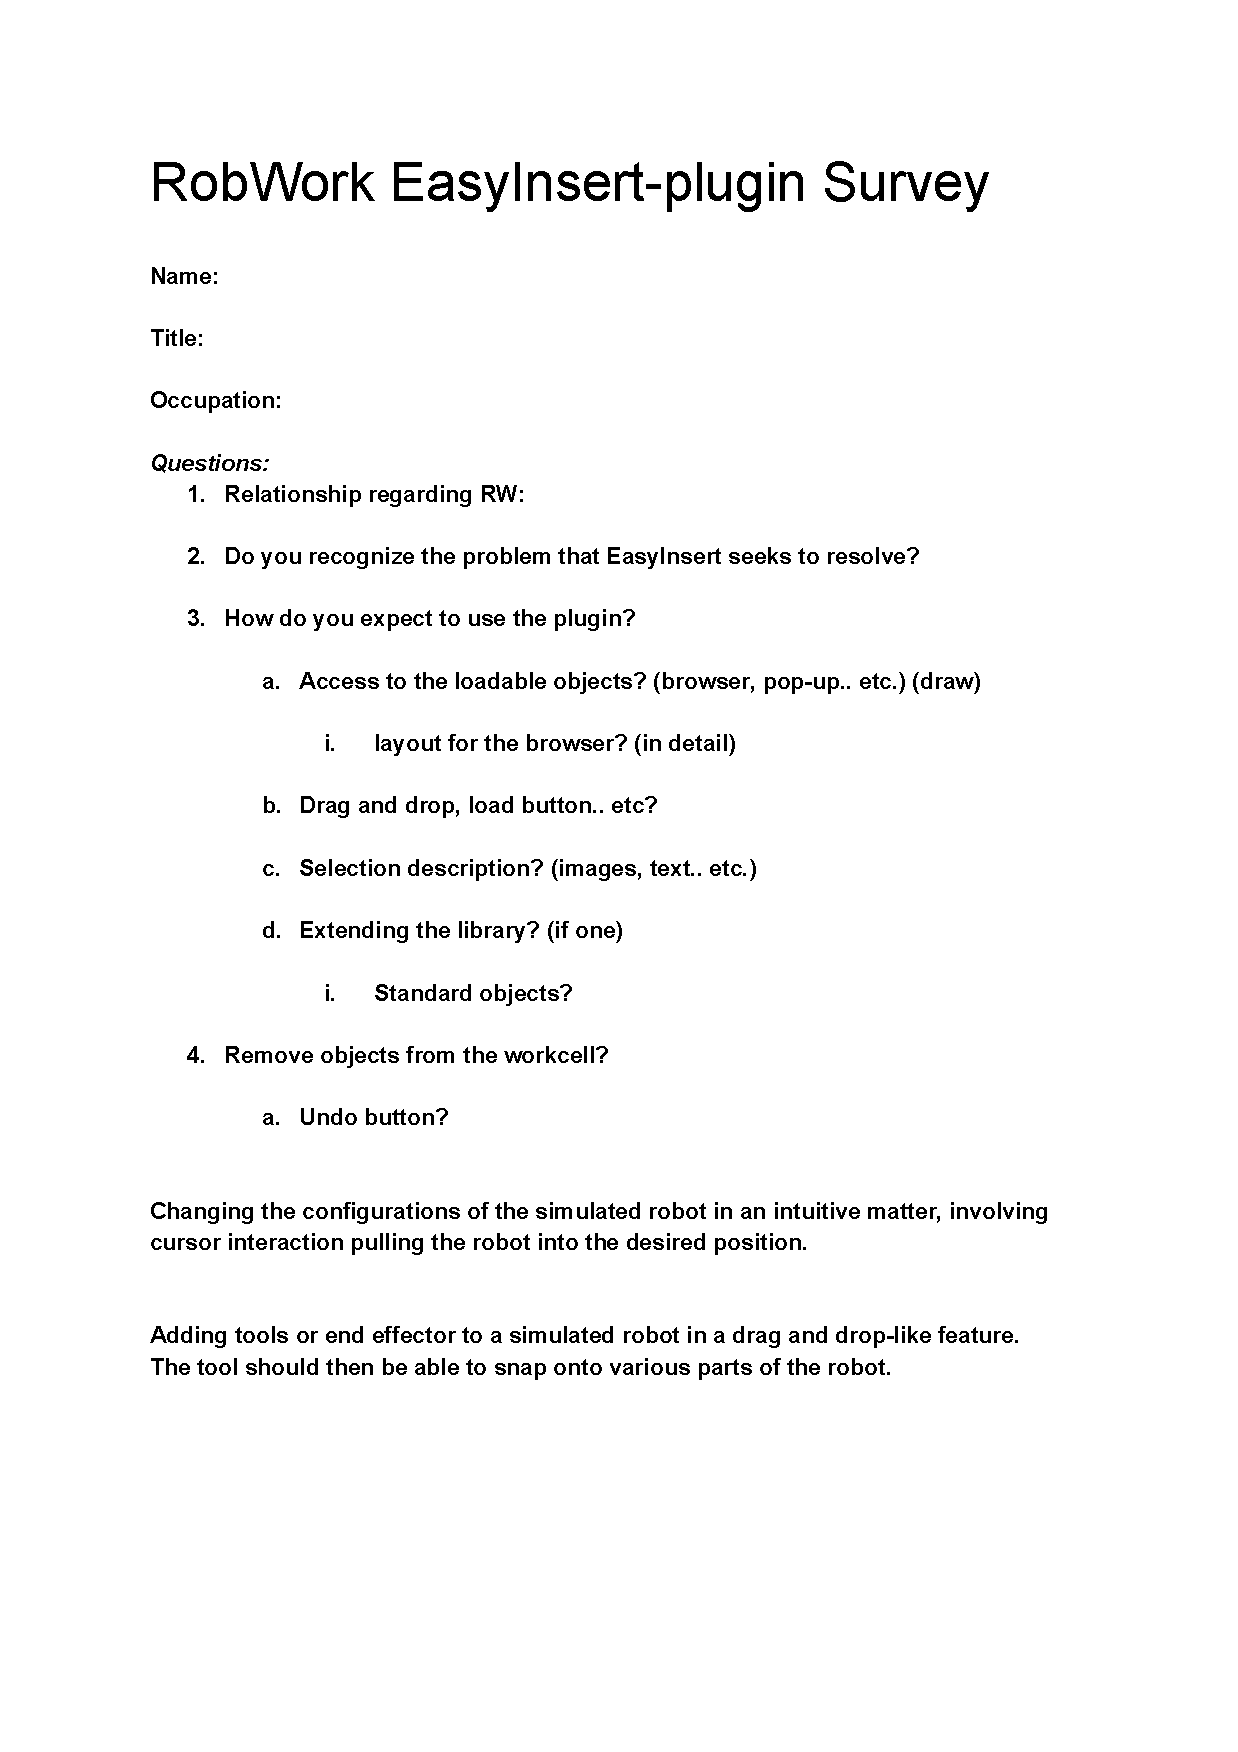
\includegraphics[trim={2.5cm 0 0 0.5cm}]{Standardfiler/Appendix/Interview.pdf}
\clearpage
\section{Use cases}
\label{app:useCases}
\subsection{Use cases for current use}
\textbf{Adding a frame/geometry to a WorkCell}

\noindent\textit{Main Success Scenario:} The user opens the XML-file describing the WorkCell in an editor. The user then writes the appropriate tag for adding the frame/geometry. The user then writes the appropriate tags for adding the additional information for the frame/geometry. The user then saves the WorkCell XML-file. The user then swaps to/ starts up RobWorkStudio. The user then loads the WorkCell from the XML-file via open in RobWorkStudio.\\

\noindent\textit{Alternate Scenarios:}

\noindent The user makes an error, the loader or parser catches this error and stops the loading process. The user is informed of the error.\\
\\

\noindent\textbf{Adding a device to a WorkCell}

\noindent\textit{Main Success Scenario:} The user opens the XML-file describing the WorkCell in an editor. The user uses the include tag to refer to the description of the device from another XML-file. The user then saves the WorkCell XML-file. The user then swaps to/ starts up RobWorkStudio. The user then loads the WorkCell from the XML-file via open in RobWorkStudio.\\

\noindent\textit{Alternate Scenarios:} 

\noindent The user manually writes the description of the device.\\

\noindent The user makes an error, the loader or parser catches this error and stops the loading process. The user is informed of the error. \\
\\

\noindent\textbf{Deleting an element}

\noindent\textit{Main Success Scenario:} The user opens the XML-file describing the WorkCell in an editor. The user deletes the tag that resembles the part the user wishes to delete. The user then saves the WorkCell XML-file. The user then swaps to/ starts up RobWorkStudio. The user then loads the WorkCell from the XML-file via open in RobWorkStudio.\\

\noindent\textit{Alternate Scenarios: }

\noindent The user makes an error, the loader or parser catches this error and stops the loading process. The user is informed of the error.\\

\clearpage
\subsection{Use cases for solution}

\noindent\textbf{Adding a frame/geometry to a WorkCell}

\noindent\textit{Main Success Scenario: }The user selects the wanted type of frame/geometry. The user then inputs the required information for the selected type of frame/geometry. The frame/geometry is then created and inserted into the WorkCell.\\

\noindent\textit{Alternate Scenarios:}

\noindent If the user supplied invalid information, the user is informed of the invalid information.\\
\\

\noindent\textbf{Adding a device to a WorkCell}

\noindent\textit{Main Success Scenario:} The user supplies the description of the device. The user then supplies the information about where the device should be placed and possibly a transform. The user also gives the device a name.\\

\noindent\textit{Alternate Scenarios:}

\noindent If the user gave the device a name that is already in use, the adding process is stopped and the user is informed of this error.\\

\noindent If the user supplied invalid information, the user is informed of the invalid information.\\
\\

\noindent\textbf{Deleting an element}
\noindent\textit{Main Success Scenario:} The user selects the element that the user wishes to delete. The user then initialises the deletion process.\\

\noindent\textit{Alternate Scenarios:}

\noindent If the user supplied invalid information, the user is informed of the invalid information.

%\titlelabel{Appendix~\thetitle\quad}
%	
%
%------------------------------------------------
% Ord- og symbolliste 	Kan pt. kun bruges med report klassen
%------------------------------------------------
%	\let\stdchapter\chapter
%	\def\chapter*#1{\stdchapter{#1}\label{symbolliste}}
%	\printnomenclature[2cm]
%	\let\chapter\stdchapter
%
%************************************************
\addtocounter{BilagSider}{\thepage}
%************************************************
\end{document}